%!TEX root=../../main.tex

\section{Backend und Infrastruktur}
\label{chapter:conceptbi}
\subsection{Einleitung}
Der Anspruch an die Infrastruktur und an das \textit{Backend} besteht darin, die Software als ganzes zu steuern und zu erhalten. Die Infrastruktur muss einfach aufzubauen und zu starten sein. Die folgenden Kapiteln erläutern nach der generellen Analyse von Lösungsmöglichkeiten im \autoref{chap:backendsota} nun einen ausgearbeiteten Plan, wie die später folgende Implementierung aussehen soll. Hierfür werden Graphiken oder Tabelle verwendet. Sie sollen ausreichend Informationen über Abläufe oder verschiedene Funktionalitäten vorgeben, um diese entsprechend daraufhin zu implementieren. Des Weiteren sollen die genormten Diagrammarten dazu dienen das komplexe \textit{Backend} und die Infrastruktur einfach und übersichtlich darzustellen, um speziell die Schnittstellenherausforderungen verständlich zu machen.
\subsection{Infrastruktur}
Die Infrastruktur enthält jegliche Dienste und Anwendungen, welche von der Software in der Projektumgebung benötigt werden. Um diese Dienste einfach mit aufbauen zu können wird eine Virtualisierung über \textit{Container} mittels \textit{Docker} umgesetzt. Diese virtuellen Instanzen, verbunden in einem \textit{Docker-Compose Stack}, werden über ein eigenes Skript gesteuert.
\subsubsection{Docker Stack}
\begin{figure}[H]
	\centering
	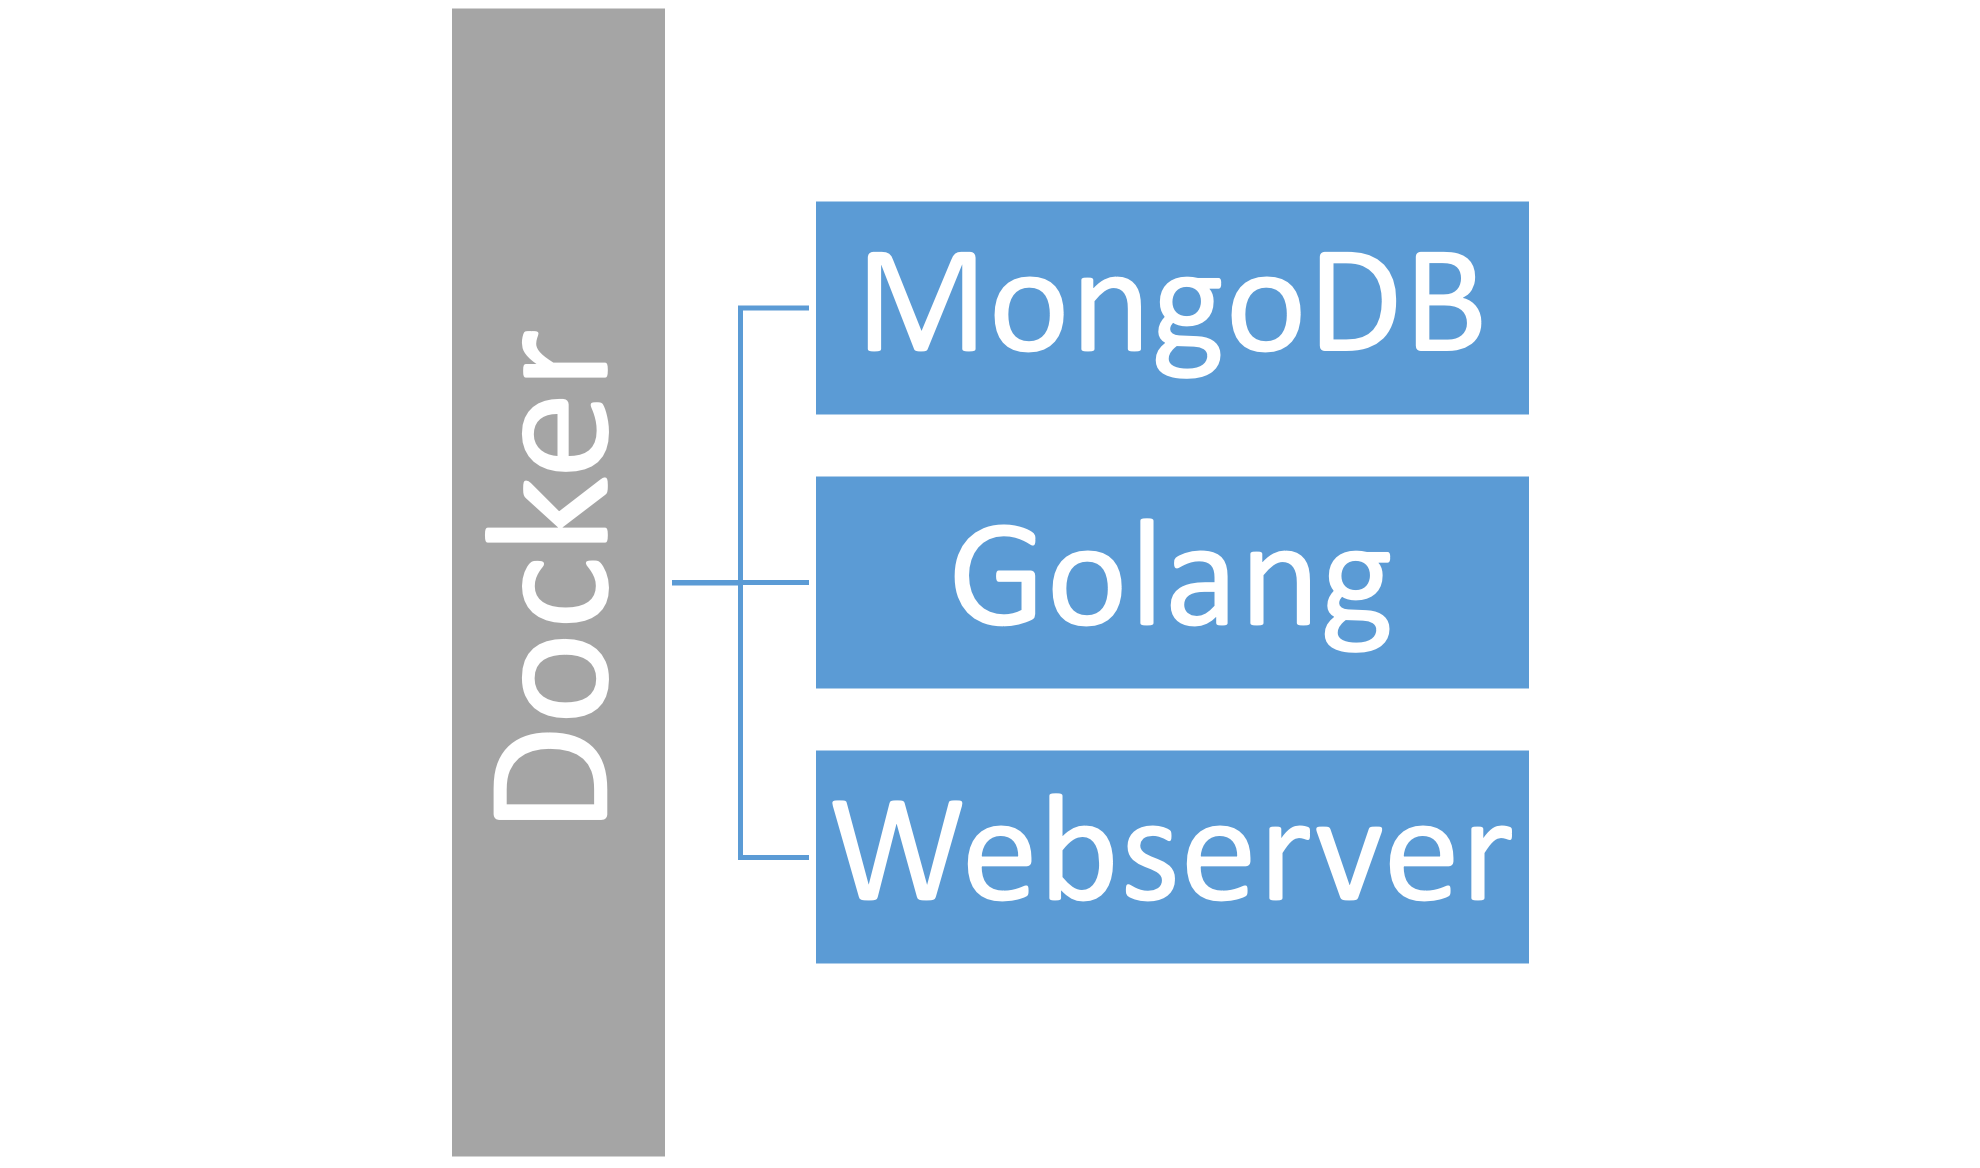
\includegraphics[width=\linewidth]{images/mbeier_konzept/docker-stack}
	\caption[\textit{Docker-Compose Stack}]{Übersicht über die \textit{Container} des \textit{Docker-Compose Stack}}
	\label{fig:docker-stack}
\end{figure}

\newpage

Diese in \textit{Docker Container} befindlichen Dienste und Anwendungen werden benötigt um die Software funktionsfähig bereitzustellen. Der automatische Aufbau dieser \textit{Container}-Infrastruktur geschieht auf Basis einer \textit{Docker-Compose} Konfiguration automatisch. \\

\textit{Docker Container} stellen eigene Umgebungen dar, welche nach dem Stoppen oftmals vollständig zerstört und gelöscht werden. Die Daten, auf die die Software und auch die anderen Anwendungen zugreifen müssen, sind jedoch über die Lebenszeit eines \textit{Docker Containers} hinaus zu persistieren. Um dies garantieren zu können, werden \textit{Volumes} in die \textit{Container} eingehängt, sodass die Daten prinzipiell außerhalb der \textit{Container} gespeichert werden und nur von außen in die Umgebungen eingehängt werden. Dies ist bei dem \textit{MongoDB Container} erforderlich um die Daten, welche in der Datenbank gespeichert werden, permanent zu speichern. Ebenso ist es erforderlich die generierten Dateien des \textit{Golang}-\textit{Backends} zu persistieren, um auf diese später wieder zugreifen zu können. Auch werden im \textit{Backend} diverse gleichbleibende Passphrasen, beispielsweise zum Signieren von Tokens, auf die gleiche Art und Weise gespeichert. \\

Die Zugangsdaten für den Nutzeraccount, welche beim Installieren abgefragt werden (siehe \autoref{fig:install}), der Datenbank werden über \textit{Dockers} \textit{Secrets}-\textit{Management} sowohl in den Datenbank-, als auch in den \textit{Golang}-\textit{Container} eingehängt, damit sich dieser zur Datenbank verbinden kann. In der Datenbank müssen initial neben den Datenbanknutzern auch die Datenbankinstanz selbst angelegt werden. Dies geschieht über ein eigenes zum Start ausführendes Skript. \\

Das \textit{Frontend} selbst besteht aus zwei Ebenen. Zu Beginn wird das \textit{Frontend} selbst kompiliert und installiert. Hierfür gibt es einen eigenen \textit{Container}, der hierfür eine Umgebung bietet. Danach wird der eigentliche \textit{Webserver}-\textit{Container} gestartet und die zuvor kompilierten Dateien werden in den neuen \textit{Container} kopiert. Ebenfalls wird eine angelegte Konfigurationsdatei, die den \textit{Webserver} Dienst weitergehend konfiguriert, in das entsprechende Verzeichnis hinzugefügt.\\

\newpage

\subsubsection{Steuerungsskript}

Das Steuerungsskript ermöglicht die genaue und einfache Steuerung der Infrastruktur.
Hierfür implementiert das Steuerungsskript folgende Submethoden mit entsprechenden Abläufen und Funktionalitäten:\\

\textbf{Installationsvorgang:}

\begin{figure}[H]
	\centering
	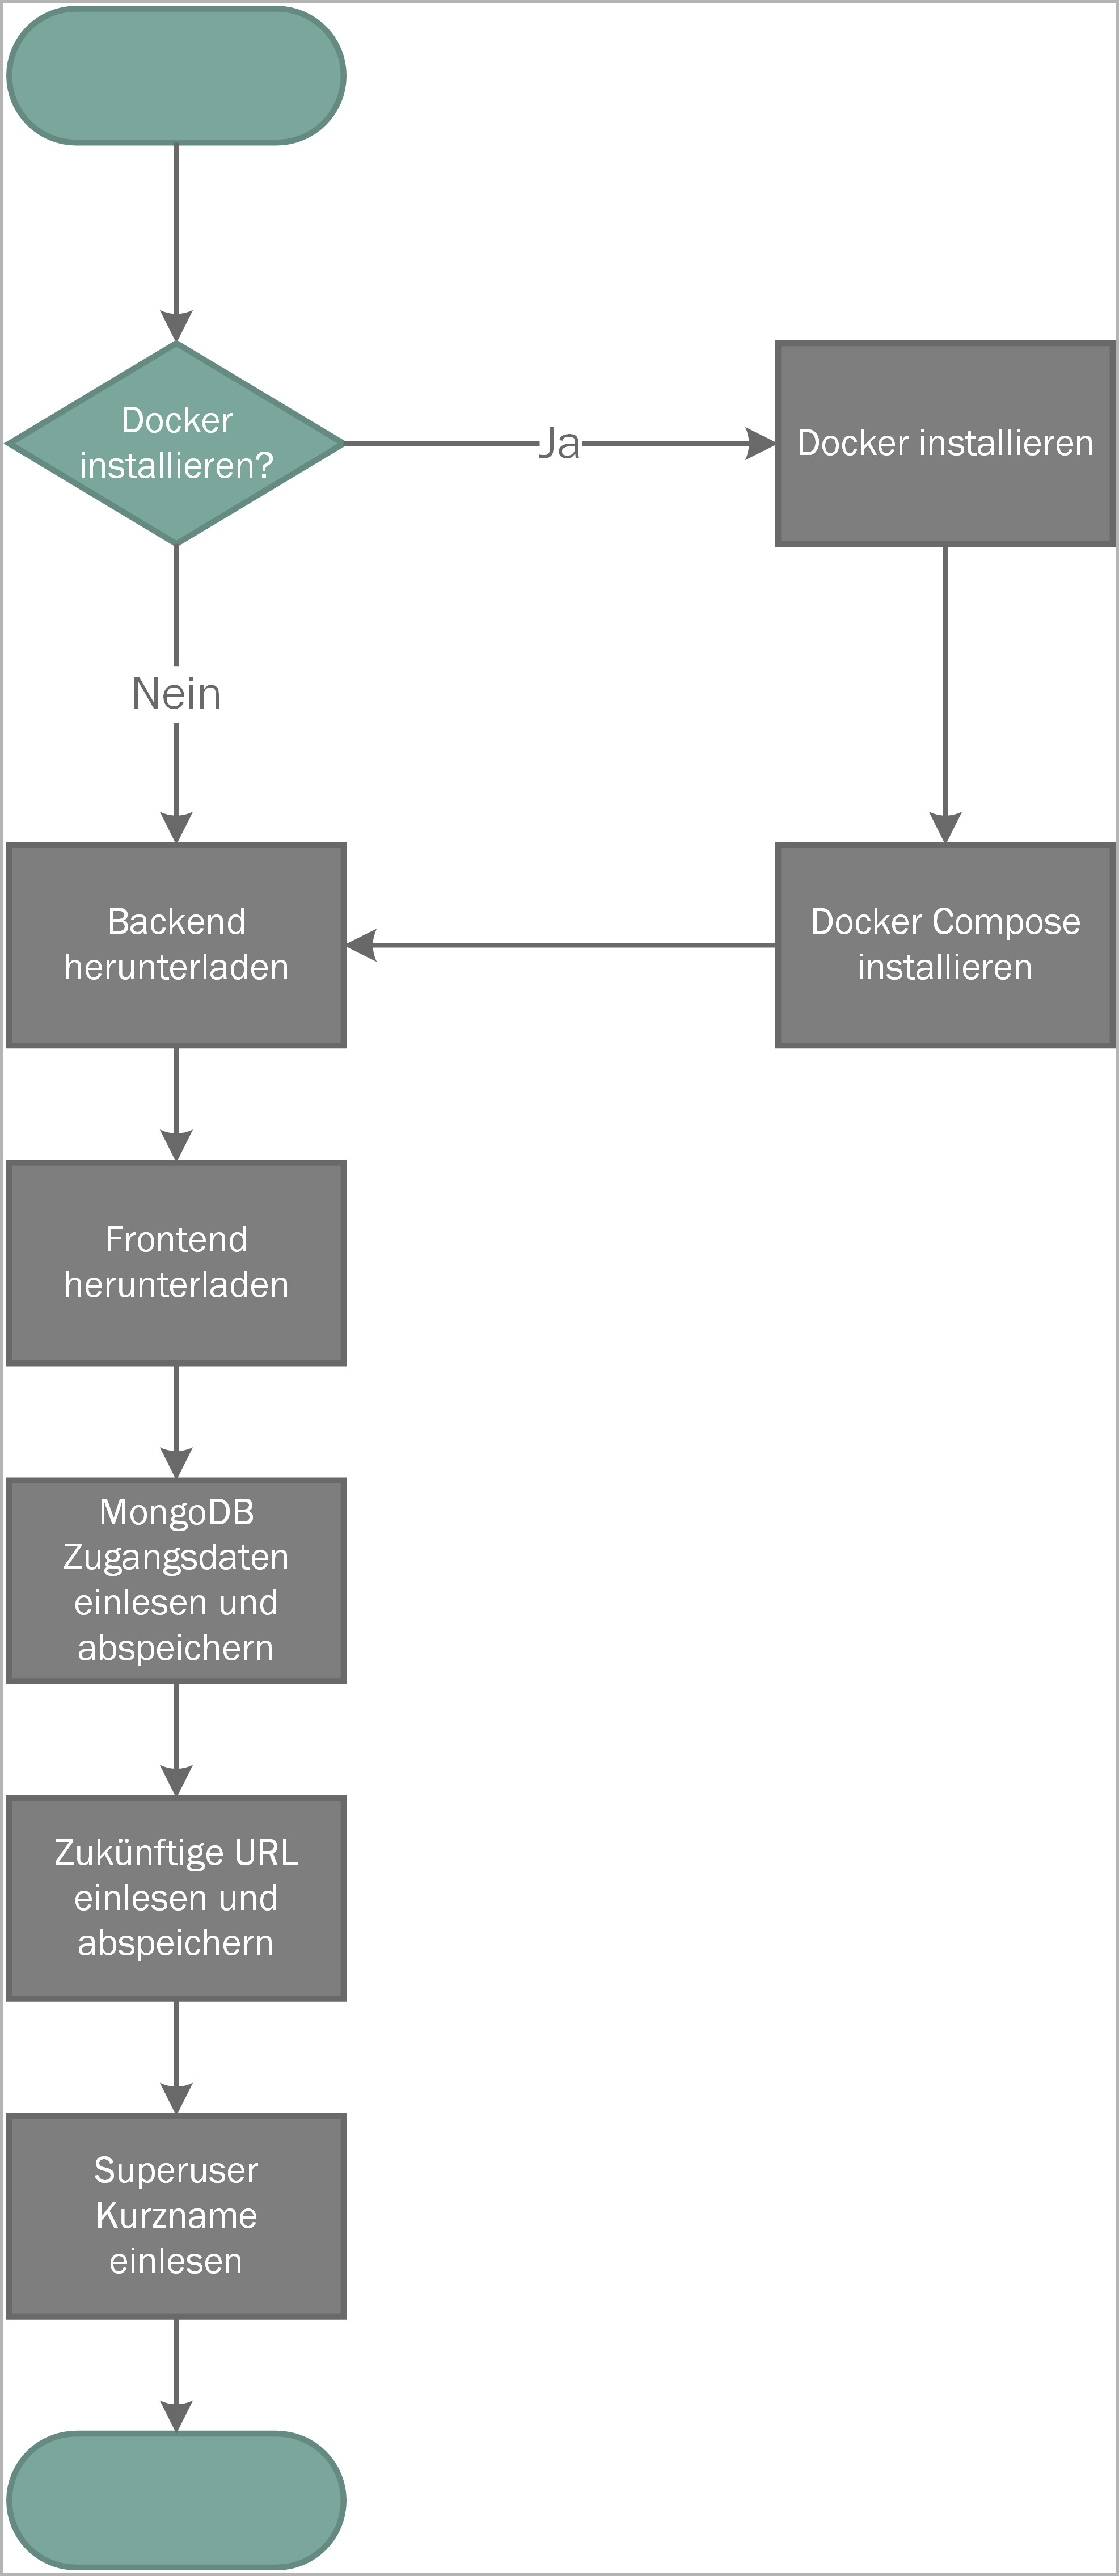
\includegraphics[width=0.5\linewidth]{images/mbeier_konzept/Install_border}
	\caption[Flussdiagramm über den Installationsvorgang]{Flussdiagramm über den Installationsvorgang}
	\label{fig:install}
\end{figure}

\newpage

Die Idee hinter der Etablierung eines Installationsvorganges soll die Einfachheit der Steuerung der Software hervorheben. Das \textit{Install}-\textit{Repository} beinhaltet hierbei lediglich eine grundlegende Ordnerstruktur und das Steuerungsskript selbst. Durch den Installationsvorgang werden die restlichen benötigten Daten automatisch heruntergeladen und installiert.

~\\~\\~\\
\textbf{Startvorgang:}

\begin{figure}[H]
	\centering
	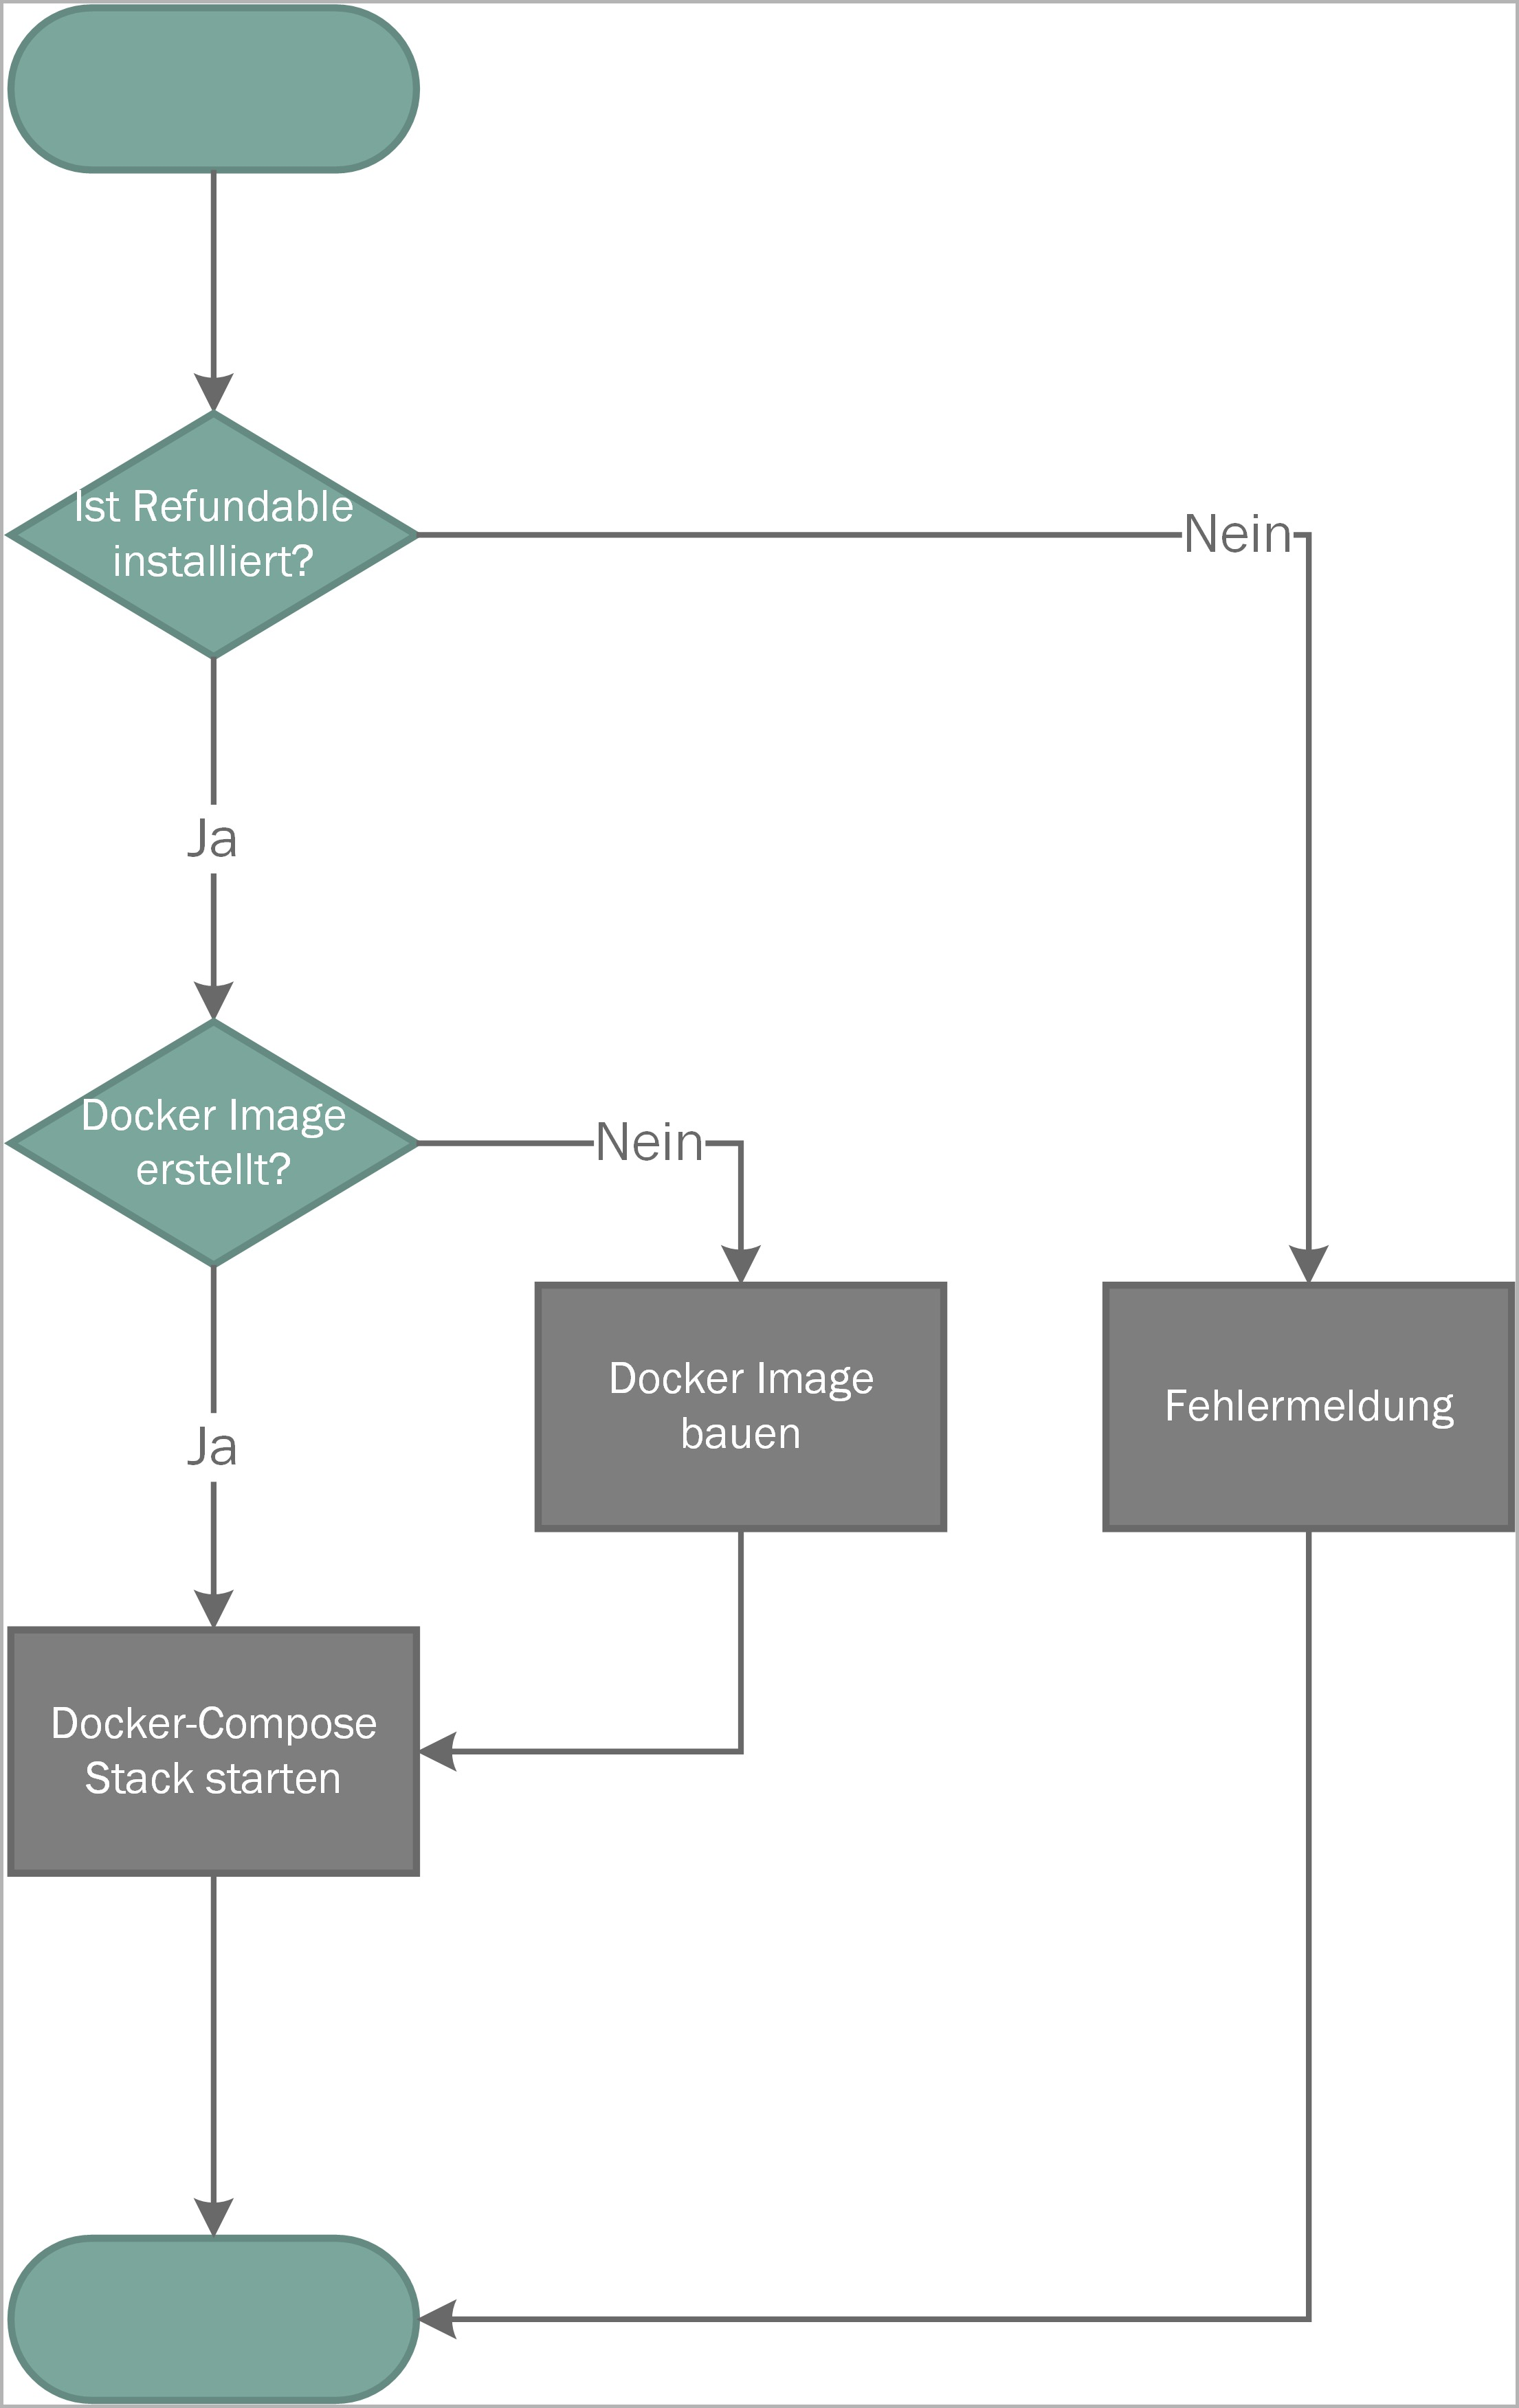
\includegraphics[width=0.5\linewidth]{images/mbeier_konzept/Start_border}
	\caption[Flussdiagramm über den Startvorgang]{Flussdiagramm über den Startvorgang}
	\label{fig:start}
\end{figure}

Der Startvorgang baut die \textit{Docker}-\textit{Images}, sofern diese noch nicht vorhanden sind, grundlegend auf Basis der installierten Dateien auf und startet daraufhin den gesamten Stack auf einmal. Voraussetzung hierfür ist, dass der Installationsvorgang bereits abgeschlossen ist und die heruntergeladenen Dateien vorhanden sind.

\newpage  

\textbf{Stoppvorgang:}

\begin{figure}[H]
	\centering
	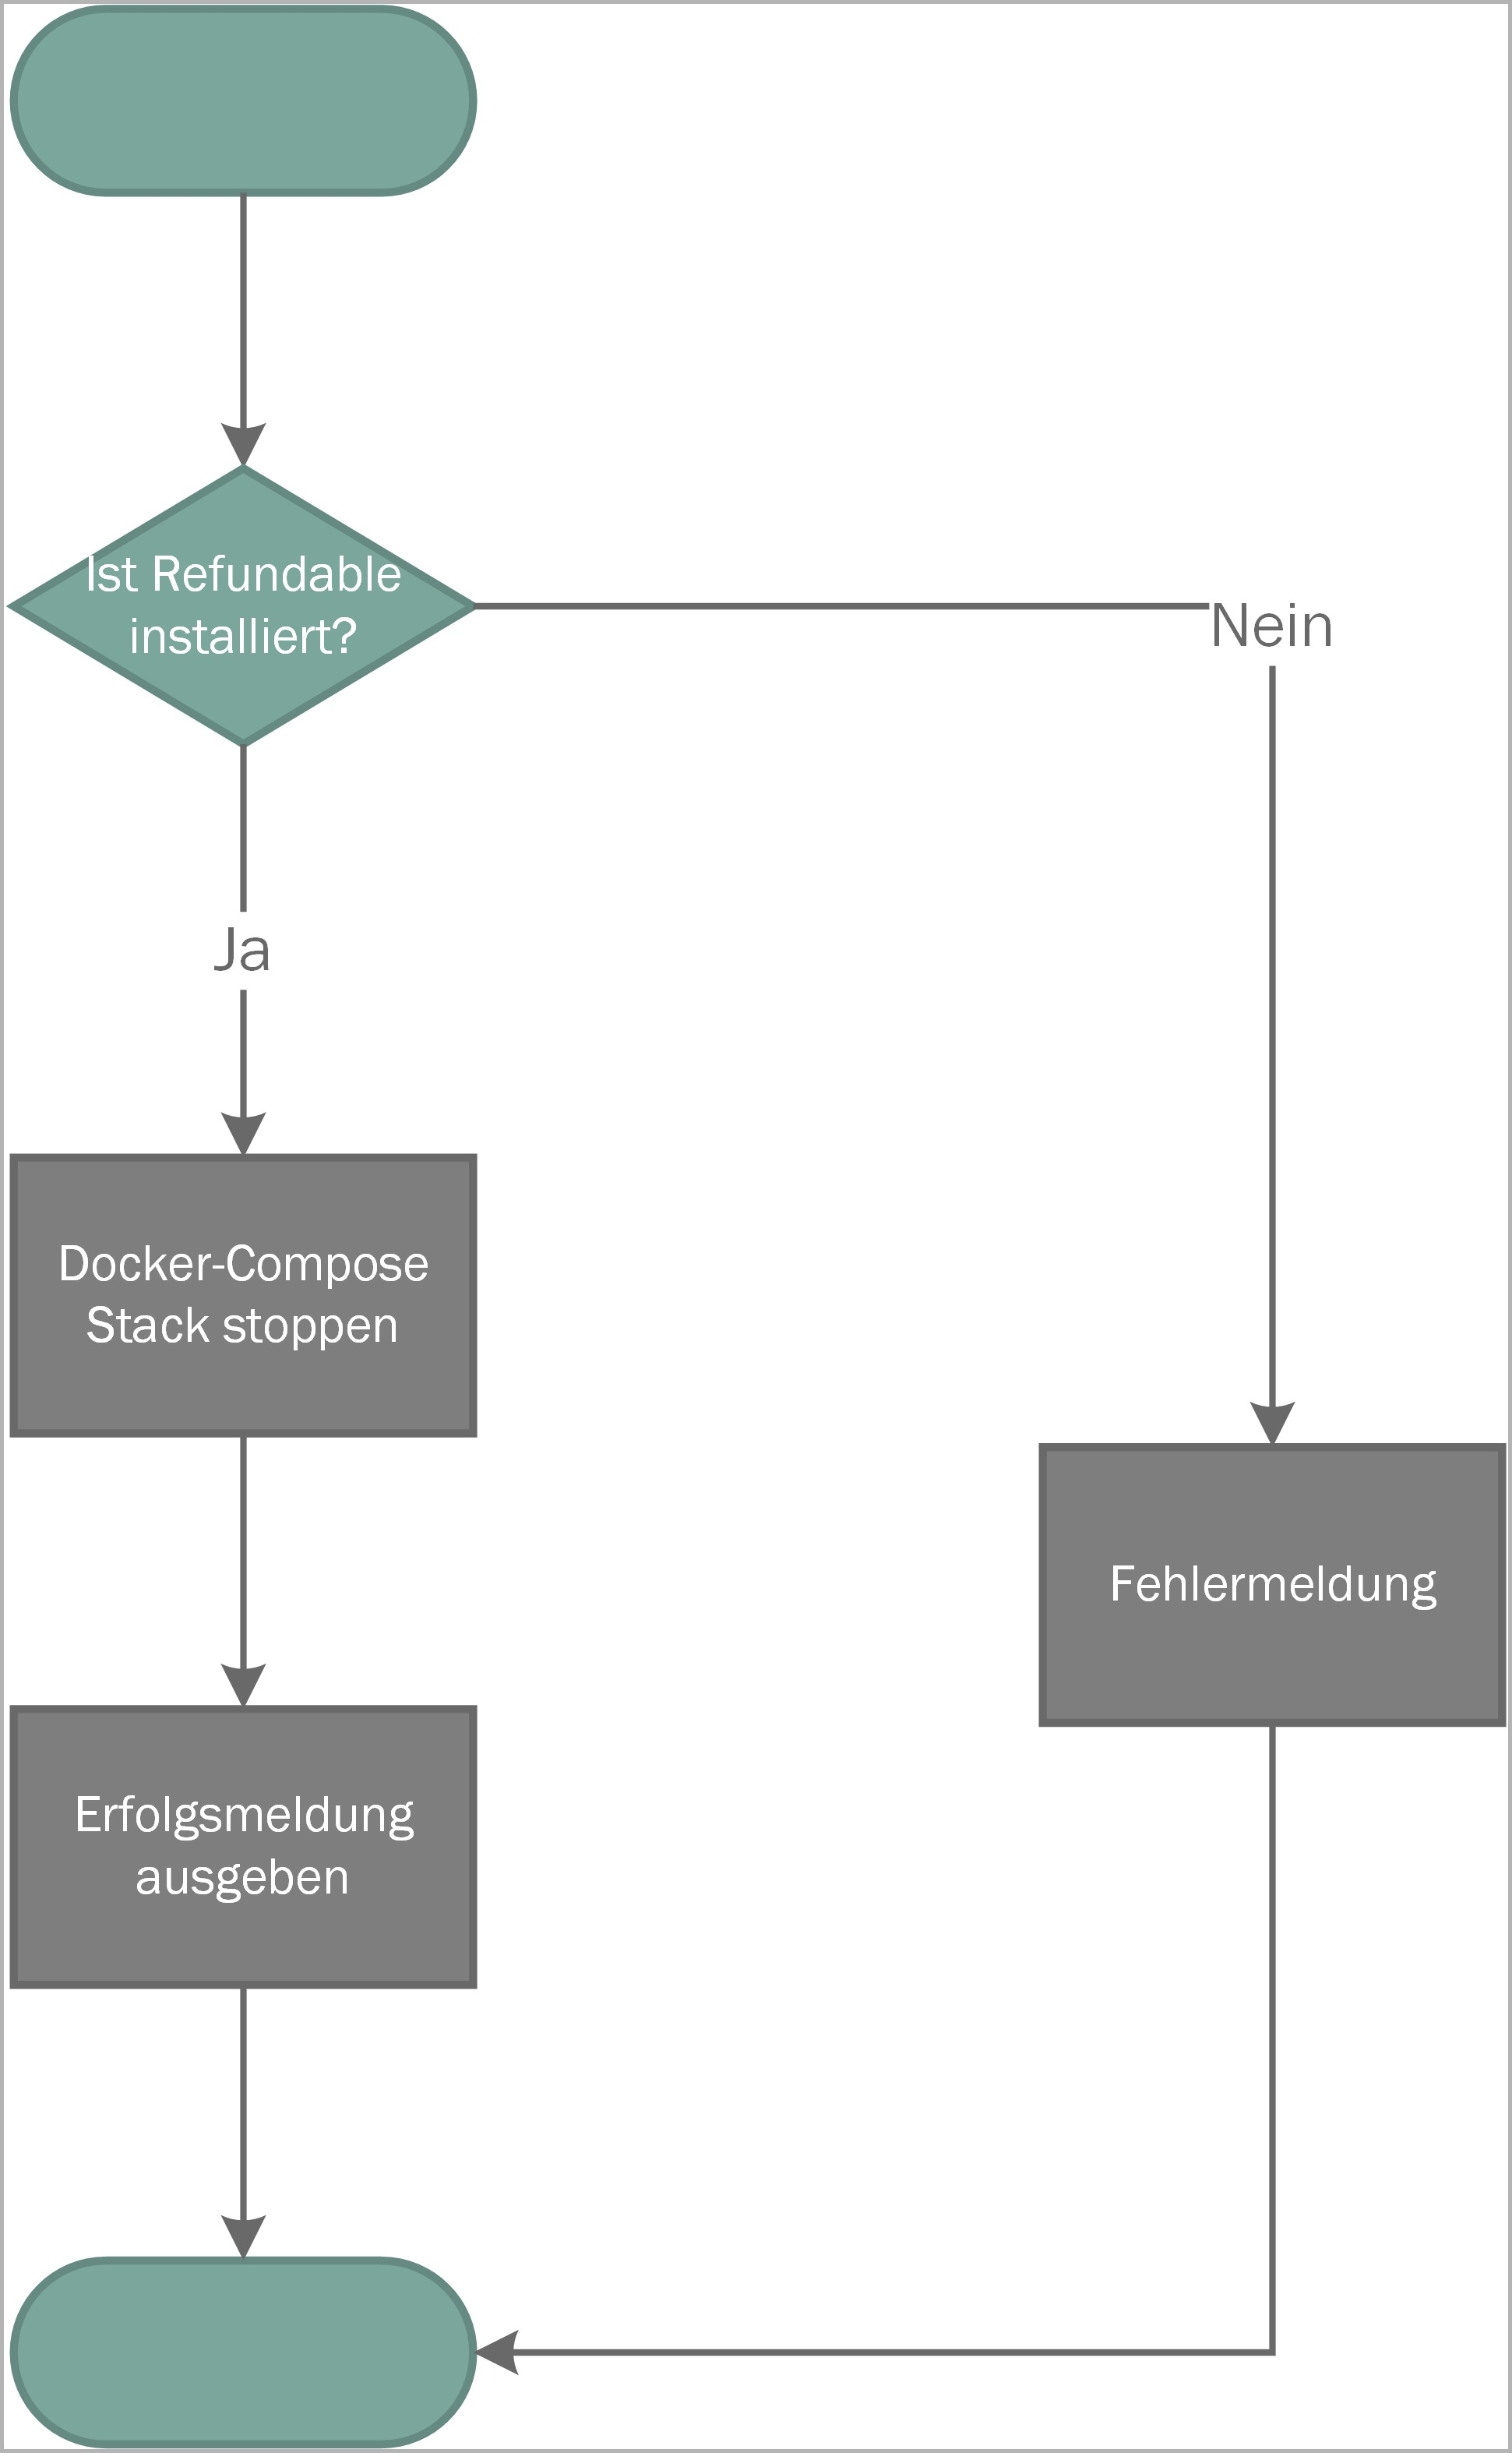
\includegraphics[width=0.5\linewidth]{images/mbeier_konzept/Stop_border}
	\caption[Flussdiagramm über den Stoppvorgang]{Flussdiagramm über den Stoppvorgang}
	\label{fig:stop}
\end{figure}

~\\
Der Stoppvorgang beendet die laufenden \textit{Docker}-\textit{Container} und entfernt diese aus der \textit{Docker} Umgebung. Dies führt dazu, dass garantiert wird, dass die sich wieder neu aufbauende Umgebung tatsächlich neu ist, und nicht nur eine alte Instanz wiederverwendet wird.

\newpage

\textbf{Neustartvorgang:}

\begin{figure}[H]
	\centering
	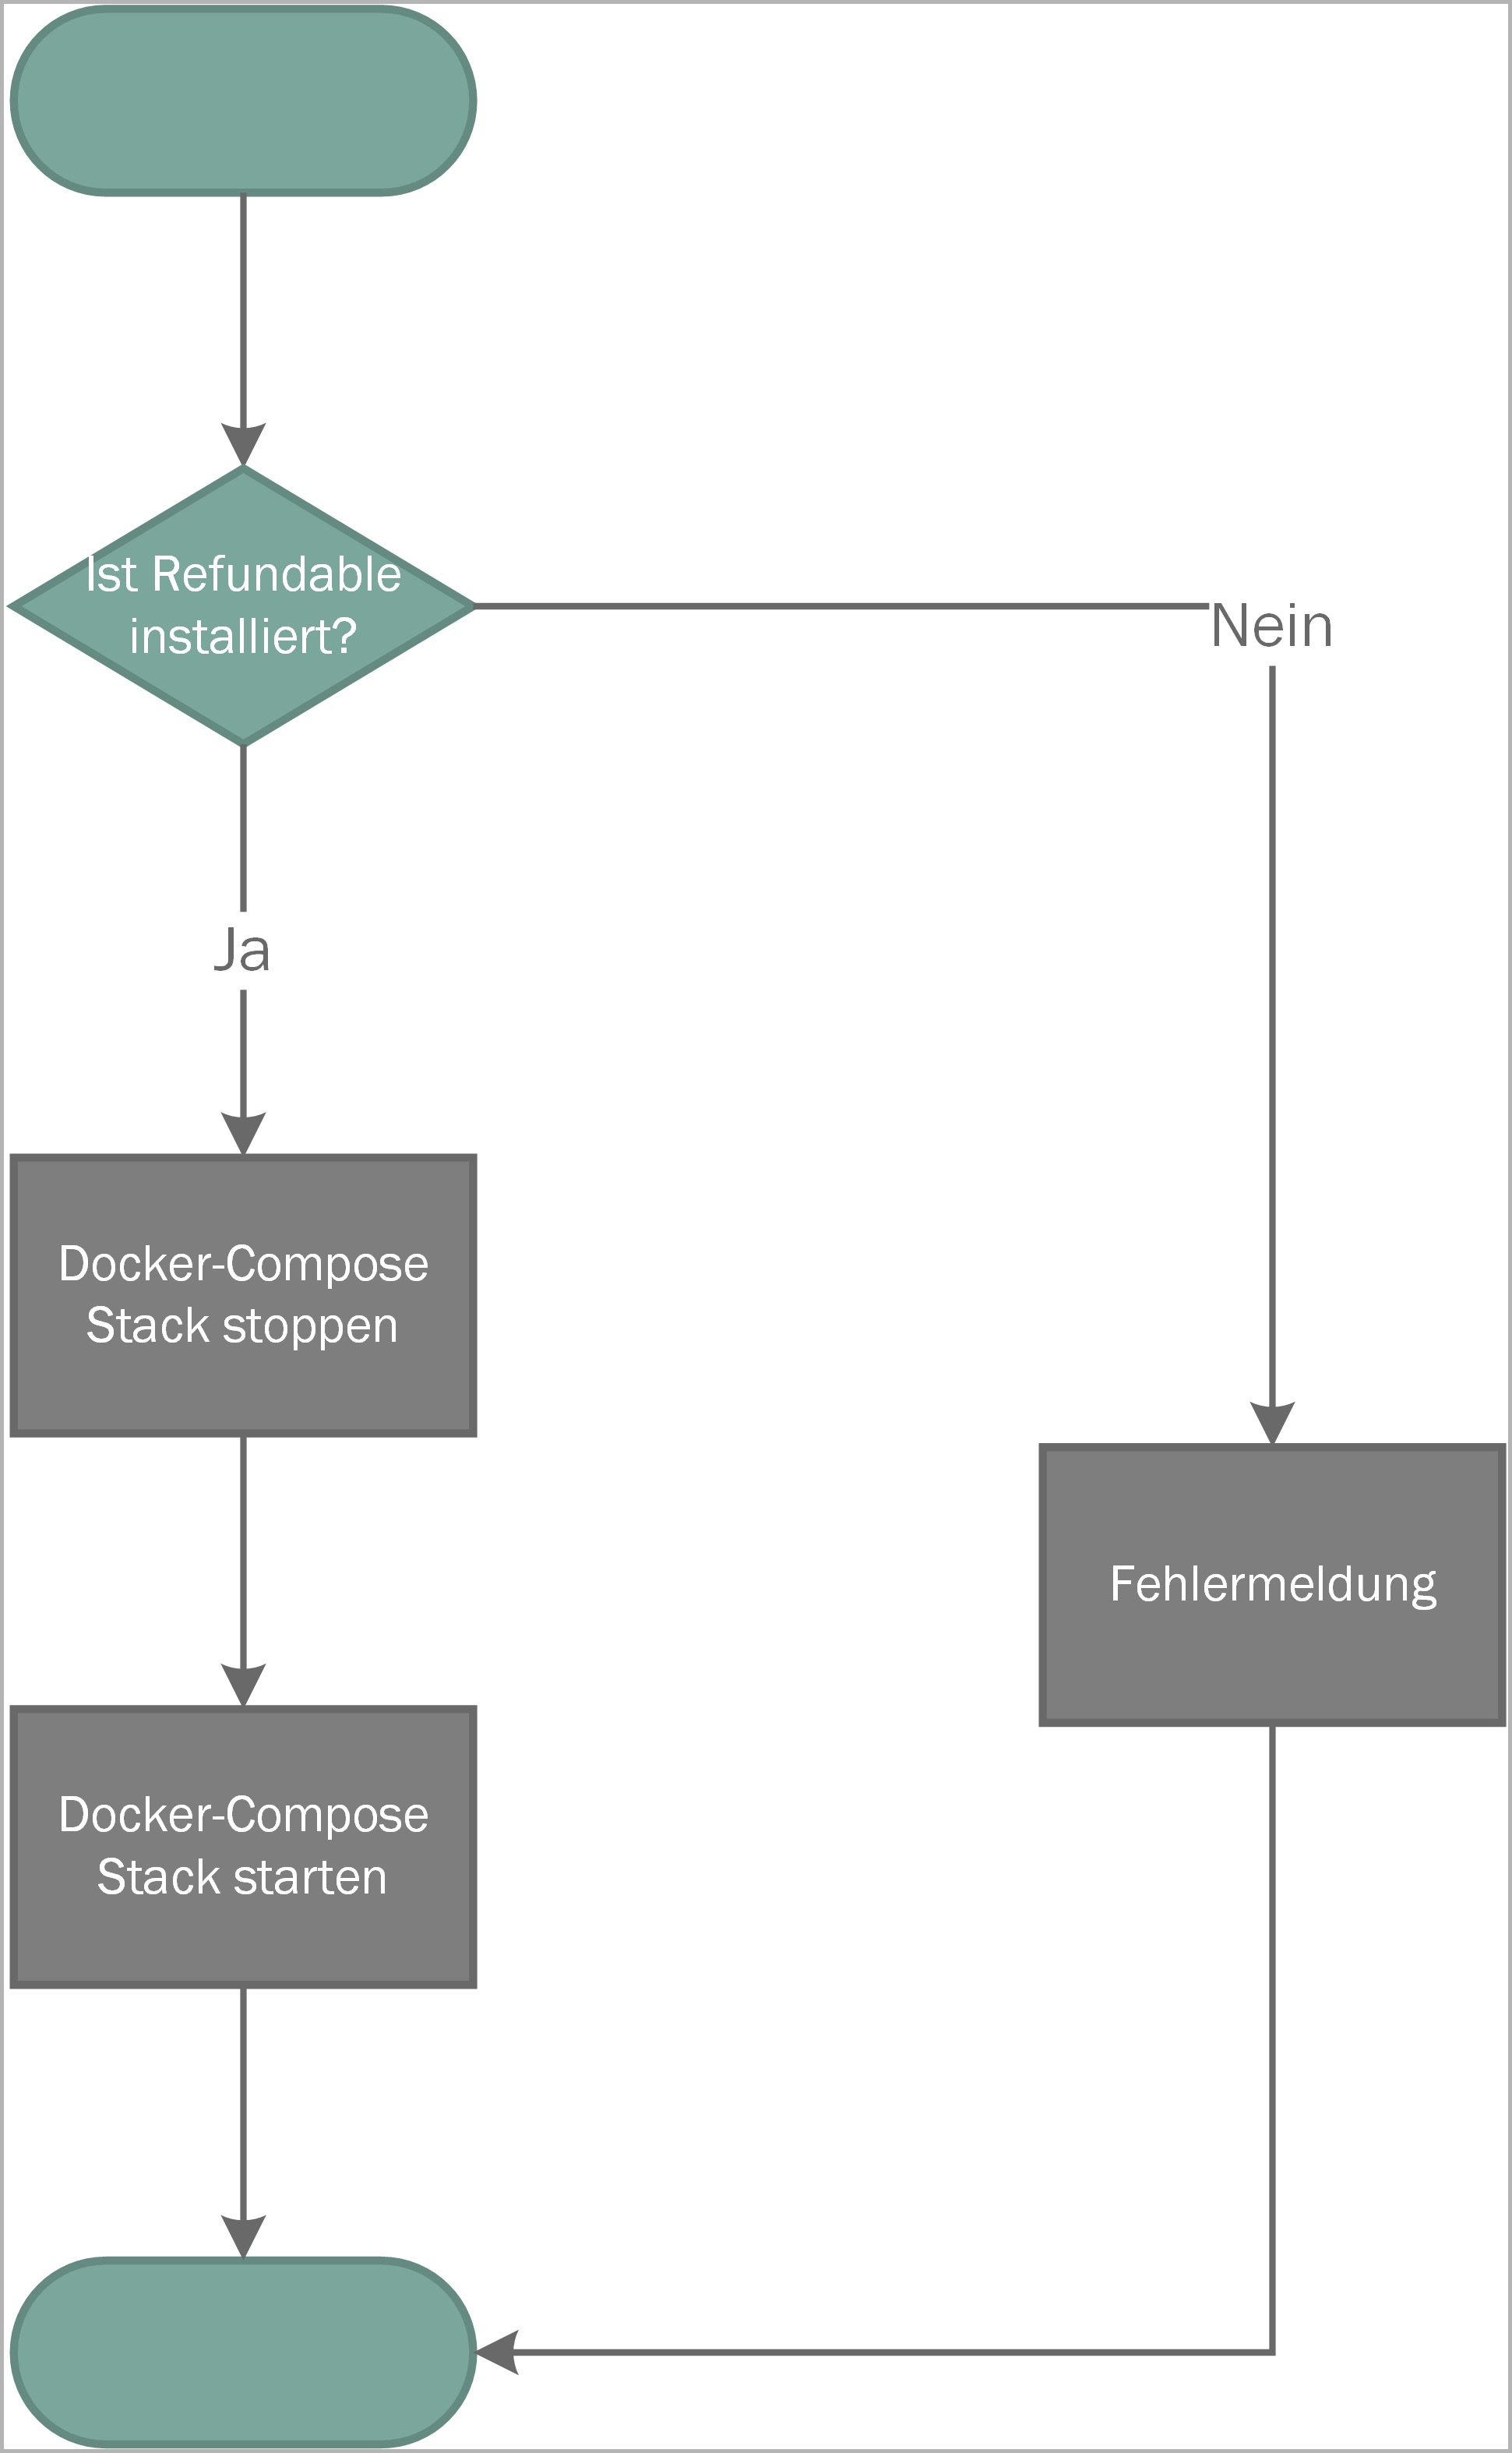
\includegraphics[width=0.5\linewidth]{images/mbeier_konzept/Restart_border}
	\caption[Flussdiagramm über den Neustartvorgang]{Flussdiagramm über den Neustartvorgang}
	\label{fig:restart}
\end{figure}
~\\
Der Neustartvorgang kombiniert den Start- und Stoppvorgang und führt diese beiden auf einmal aus. Er wird hauptsächlich dafür genutzt, um neue Konfigurationen, welche nur beim Start des Systems eingelesen werden, von der Software übernehmen zu lassen.

\newpage

\textbf{Aktualisierungsvorgang:}

\begin{figure}[H]
	\centering
	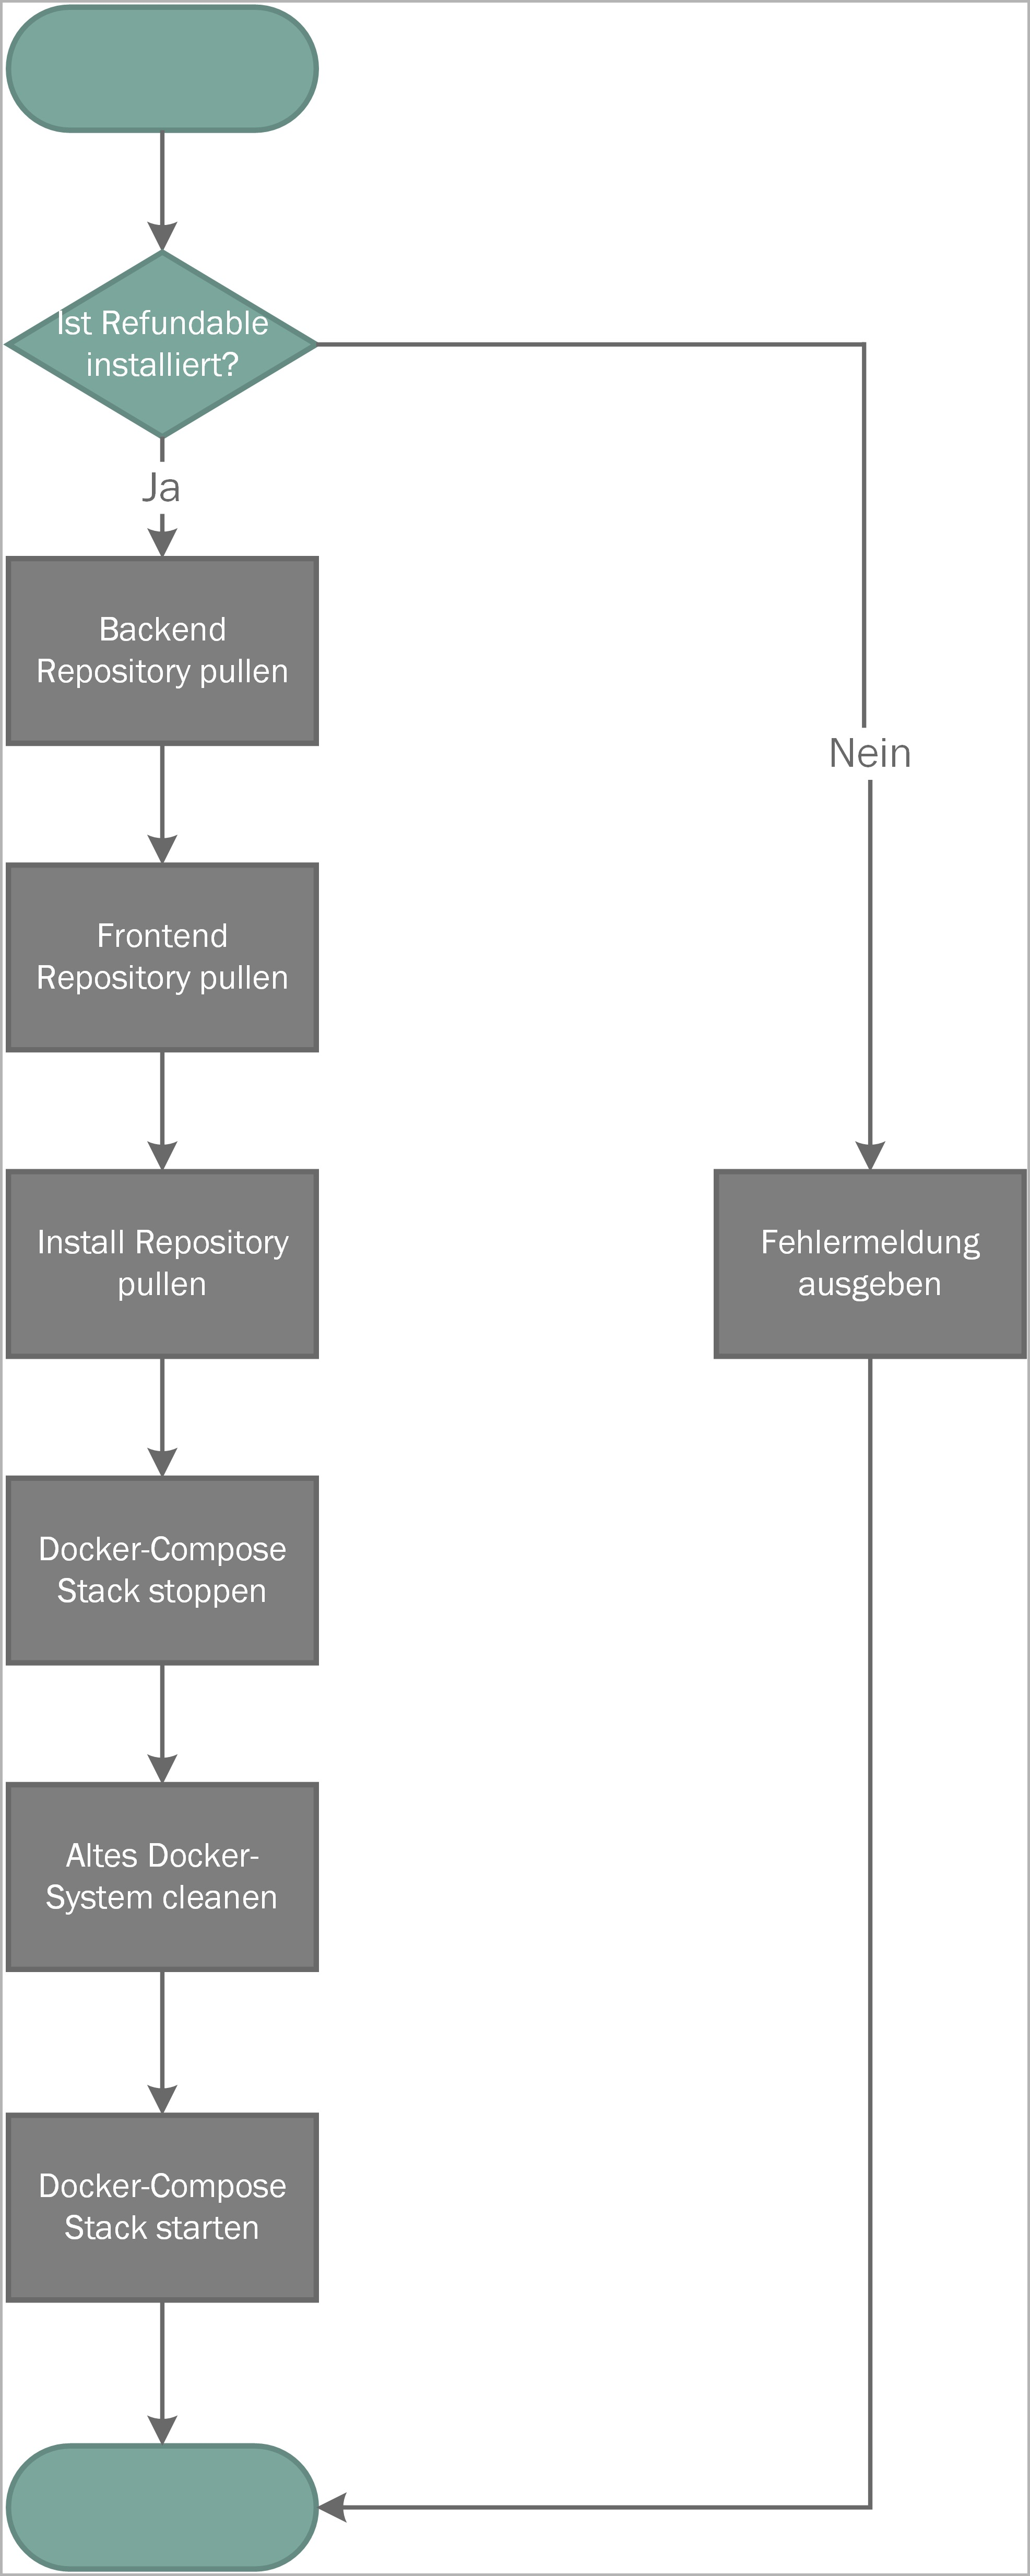
\includegraphics[width=0.47\linewidth]{images/mbeier_konzept/Update_border}
	\caption[Flussdiagramm über den Aktualisierungsvorgang]{Flussdiagramm über den Aktualisierungsvorgang}
	\label{fig:update}
\end{figure}
~\\
Der Aktualisierungsvorgang ist dem Installationsvorgang sehr ähnlich. Da es sich bei den installierten Dateien um solche aus \textit{Git}-\textit{Repositories} handelt, können diese auch einfach aktualisiert werden. Daraufhin wird nur noch ein Neustart des Systems durchgeführt.

\newpage

\textbf{Bereinigungsvorgang:}

\begin{figure}[H]
	\centering
	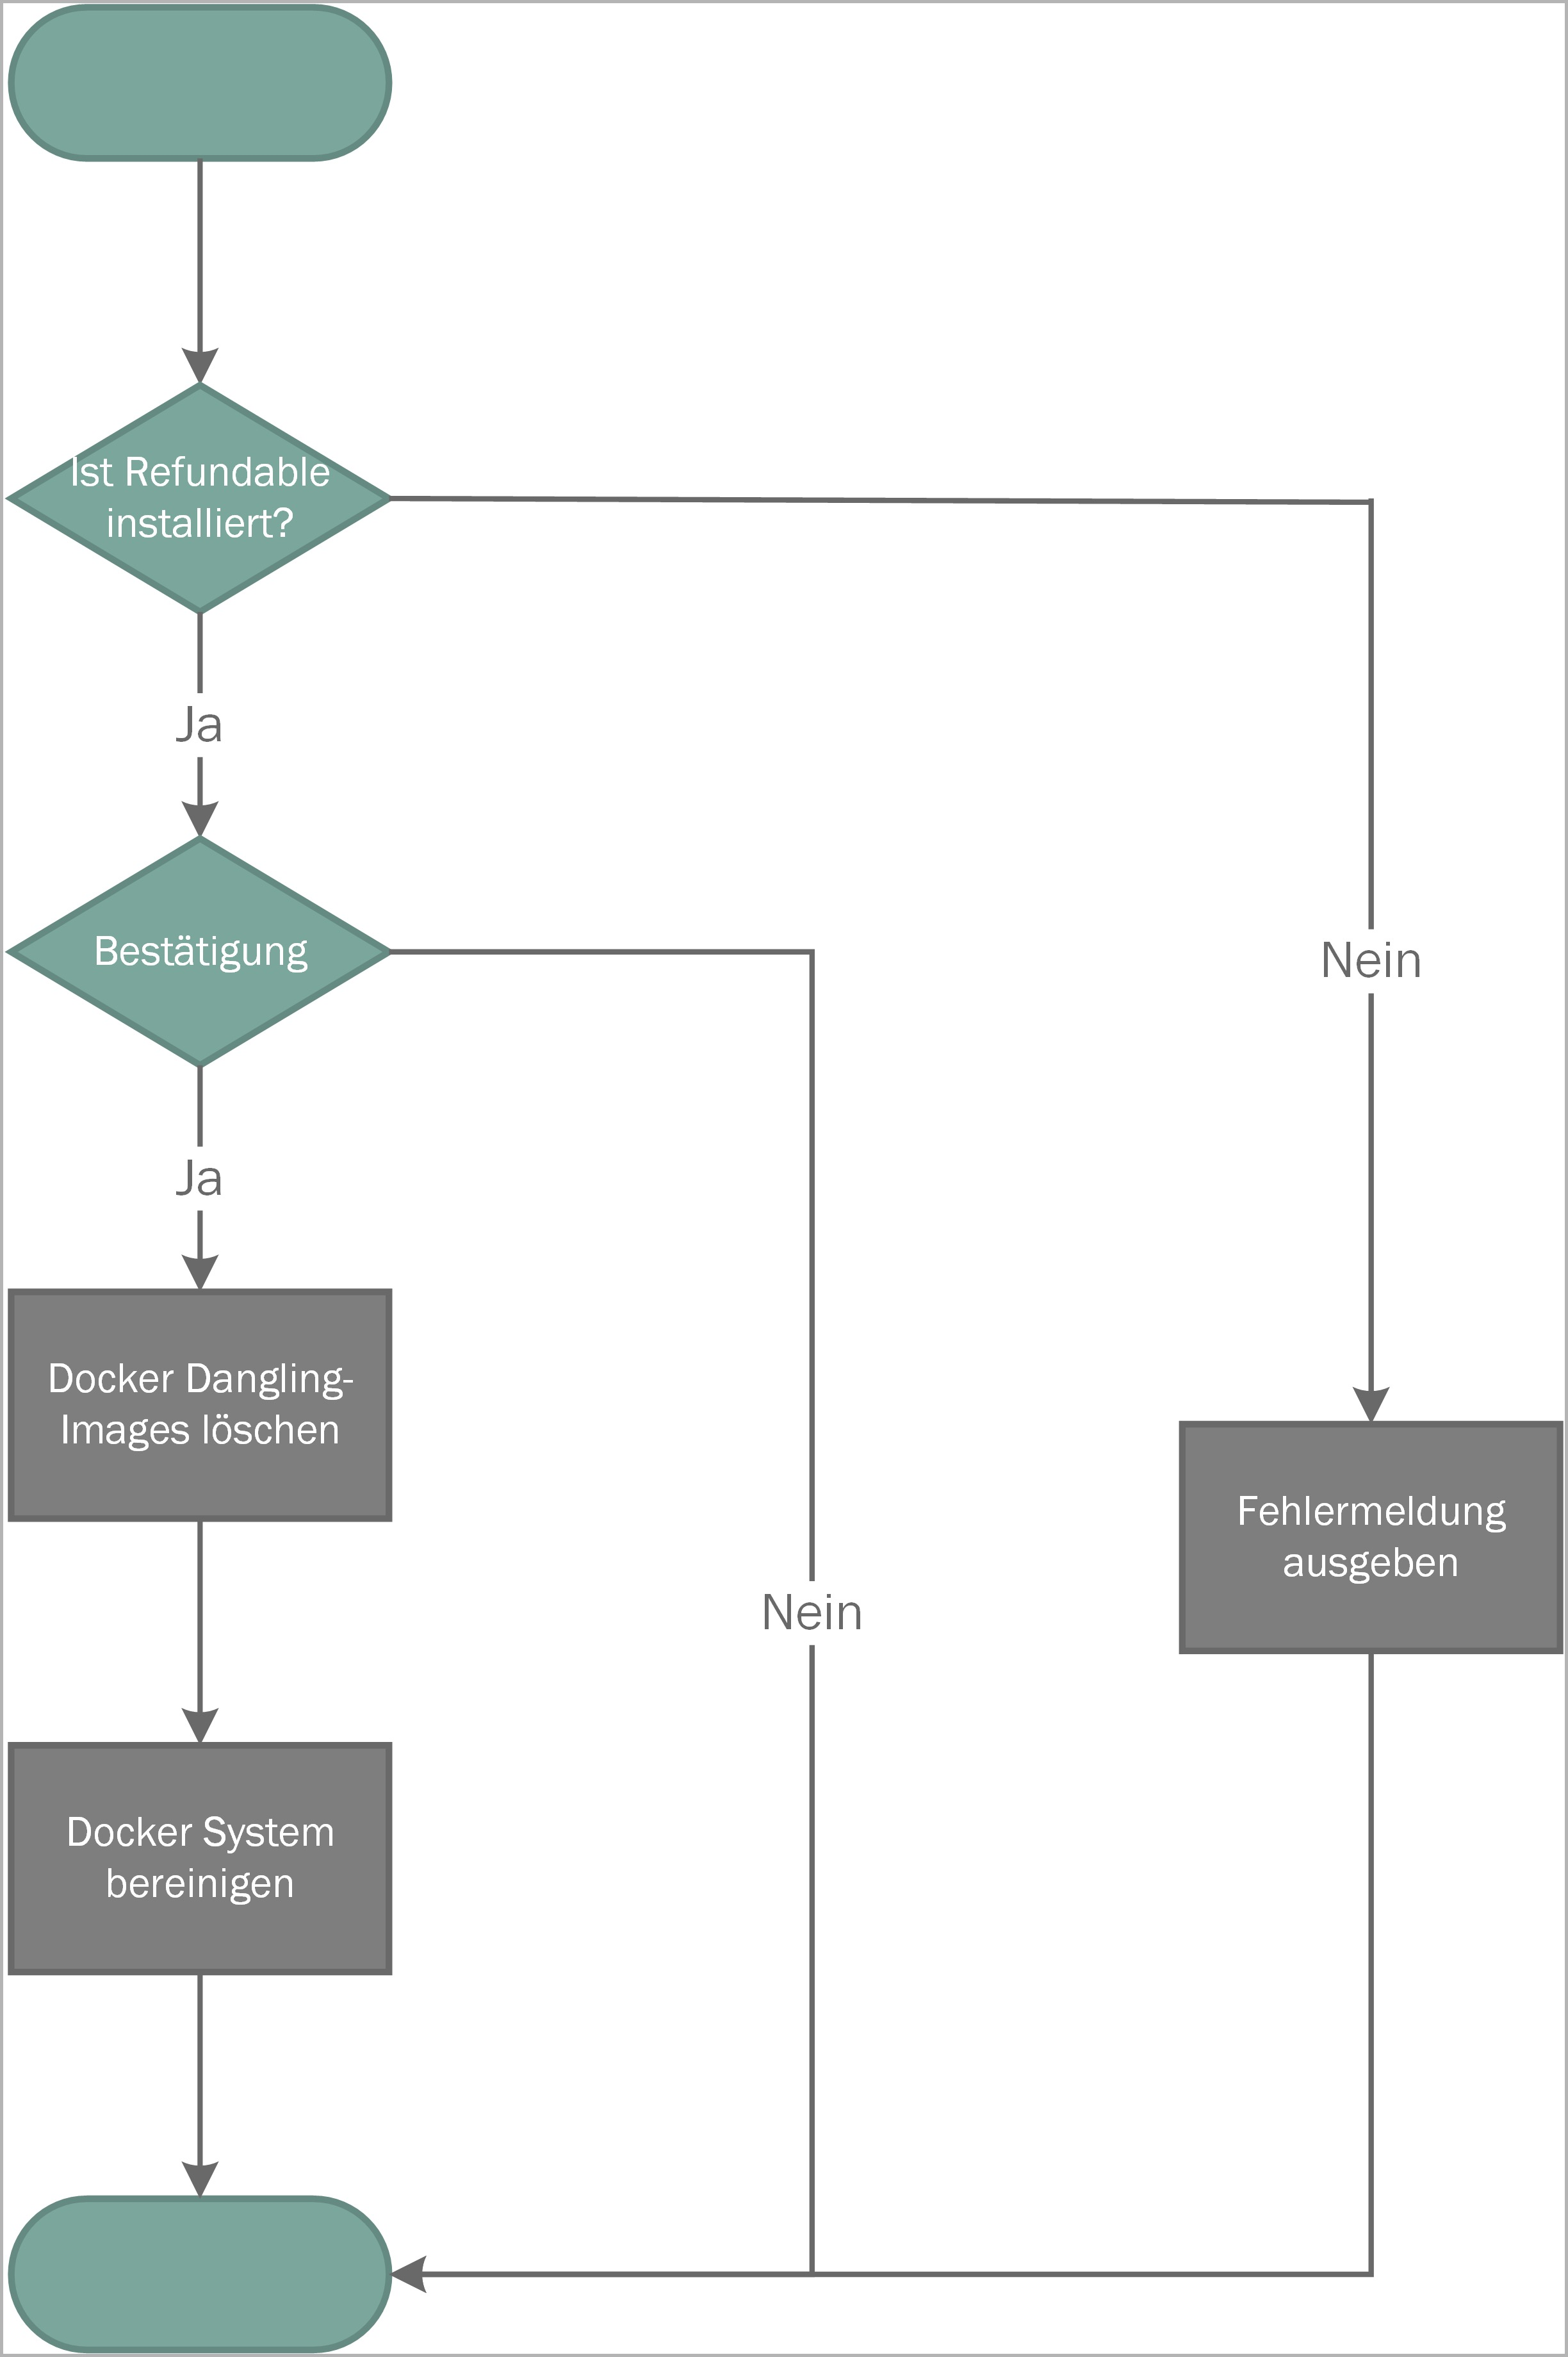
\includegraphics[width=0.55\linewidth]{images/mbeier_konzept/Clean_border}
	\caption[Flussdiagramm über den Bereinigungsvorgang]{Flussdiagramm über den Bereinigungsvorgang}
	\label{fig:clean}
\end{figure}
~\\
Der Bereinigungsvorgang nutzt die \textit{Docker} Funktionen zum Löschen von nicht mehr benutzten \textit{Docker} Images (\textit{Dangling Images}). Nachdem werden die nicht mehr benutzten Ressourcen über die entsprechende \textit{Docker}-Funktion aus dem System und der \textit{Docker} Umgebung entfernt.

\newpage

\textbf{Deinstallation:}

\begin{figure}[H]
	\centering
	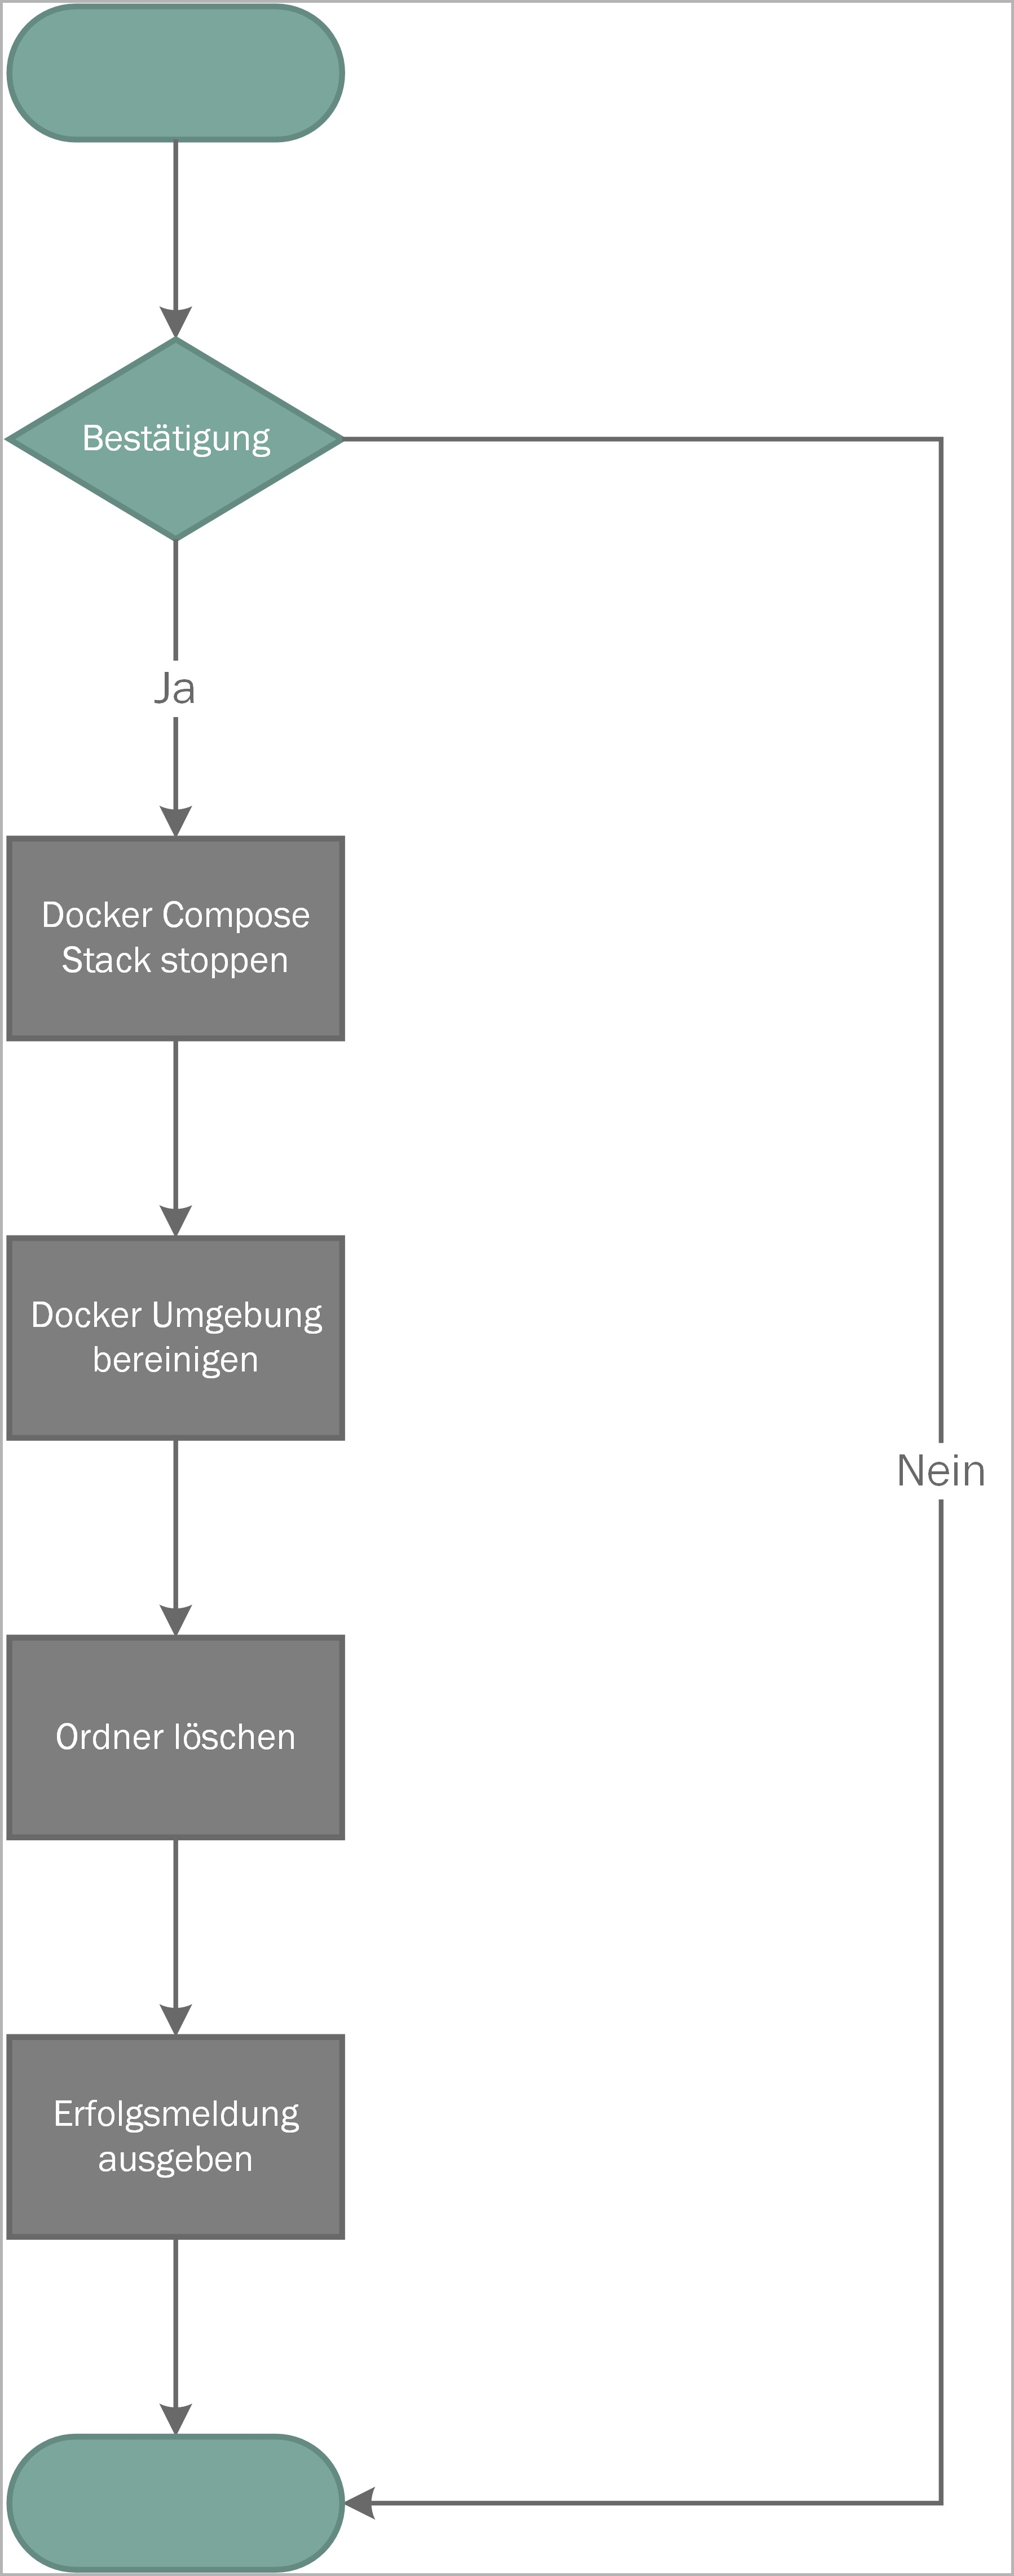
\includegraphics[width=0.48\linewidth]{images/mbeier_konzept/Purge_border}
	\caption[Flussdiagramm über die Deinstallation]{Flussdiagramm über die Deinstallation}
	\label{fig:purge}
\end{figure}
~\\
Der Vorgang hinter der Deinstallation löscht jegliche Information der Software aus der \textit{Docker} Umgebung und auch alle Dateien, welche mit den Diensten assoziiert sind.

\newpage

\subsection{Datenmodell}

Auf Basis der zu erstellenden Anträge und der allgemeinen Nutzerverwaltung wurde folgendes Datenmodell entwickelt. Darin wurde speziell darauf geachtet, dass jegliche Information auch wirklich dort zu finden ist, wo sie auch auf einem papierenen Antrag zu finden wäre. 

\begin{figure}[H]
	\centering
	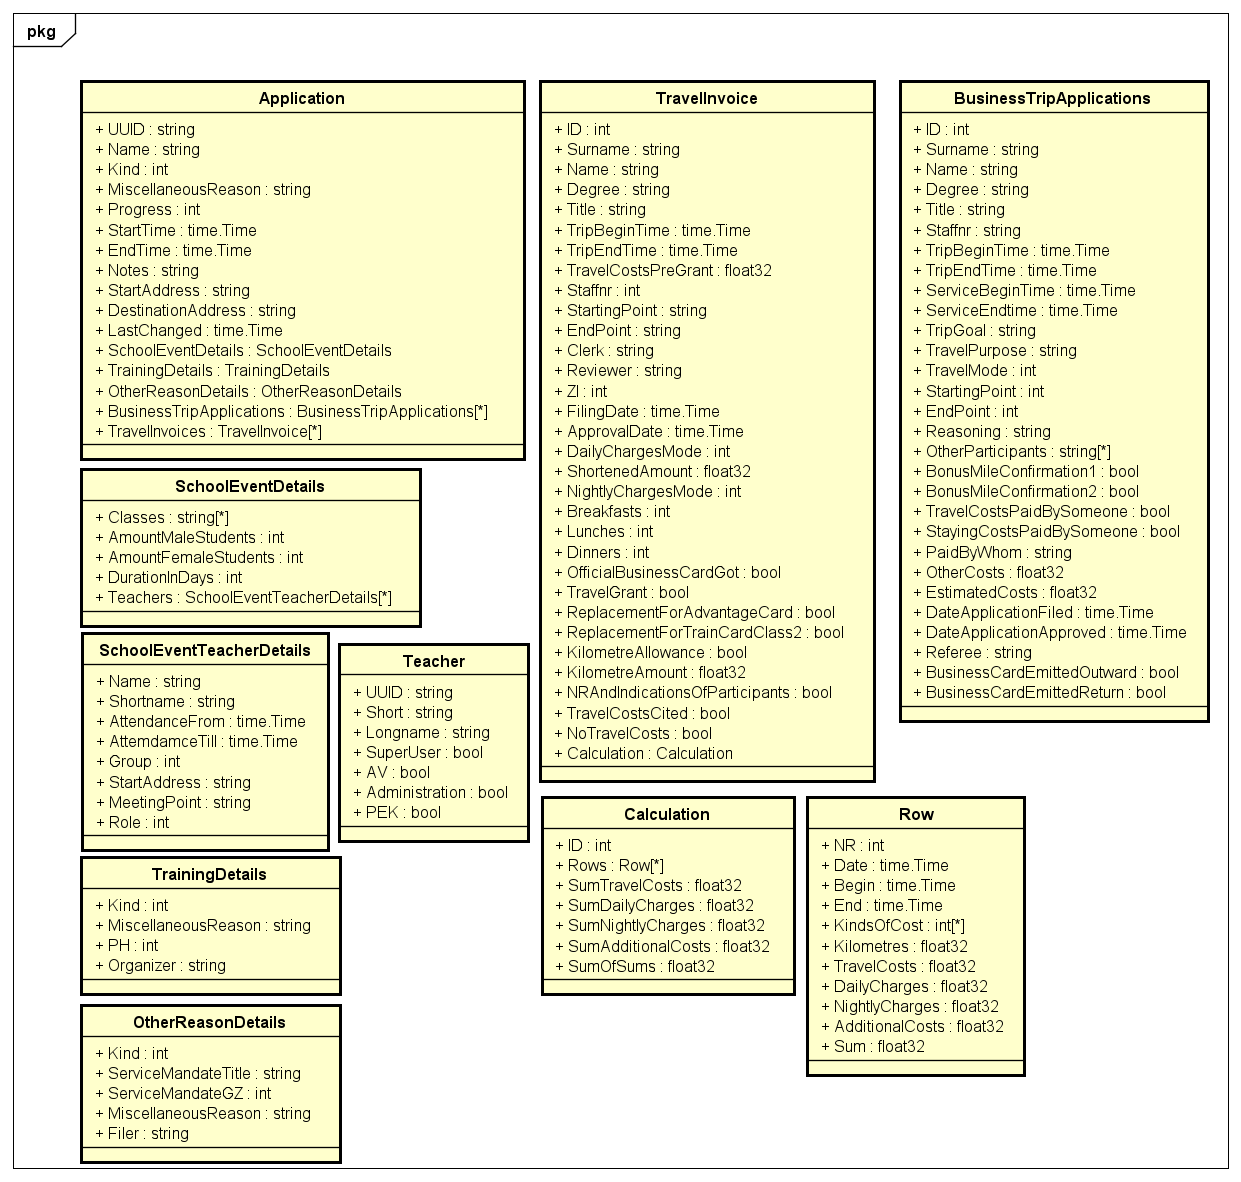
\includegraphics[width=\linewidth]{images/mbeier_konzept/Datamodel}
	\caption[Zentrales Datenmodell]{Das zentrale Datenmodell beinhaltet jegliche Daten, die von der Software benötigt werden.}
	\label{fig:datamodel}
\end{figure}

Insgesamt gibt es zehn verschiedene Datenstrukturen, wobei hierbei neun die eigentlichen Anträge inklusive Subinformationen widerspiegeln und einer die Lehrkraft-Datenstruktur, welche das Schlüsselelement der Nutzerverwaltung darstellt.

\newpage

\subsection{REST-Schnittstelle}

 erstellt. Diese sind in sich abgeschlossene Vorgänge, welche sich jeweils immer auf eine Aufgabe beschränken. Im folgenden Kapitel sind alle geplanten \textit{Endpoints} beschrieben.

\subsubsection{Endpoints}
\label{chapter:endpoints}

Die folgende Tabelle beschreibt die geplanten \textit{Endpoints}, wobei  sie jeweils mit der Protokollmethode (\textit{GET}, \textit{POST}, \textit{PUT} oder \textit{DELETE}), dem Pfad zum \textit{Endpoint}, einer kurzen Beschreibung, Rückgaben, Eingaben und dem Erfordernis eines Tokens beschrieben werden.

\captionof{table}[\textit{REST}-\textit{Endpoints} 1]{Übersicht \textit{REST}-\textit{Endpoints}: Teil 1}
\label{table:endpoints1}
\begin{table}
	\centering
	\begin{tabular}{|l|l|l|l|l|}
		\hline
		\multicolumn{1}{|c|}{\textbf{Methode}} & \multicolumn{1}{c|}{\textbf{Endpoint}}                                                  & \multicolumn{1}{c|}{\textbf{Beschreibung}}                                                                  & \multicolumn{1}{c|}{\textbf{\begin{tabular}[c]{@{}c@{}}Rückgabe\\ (Erfolg)\end{tabular}}} & \multicolumn{1}{c|}{\textbf{Eingabe}}                                                                          \\ \hline
		
		
		POST                                   & /login                                                                                  & Loggt eine Lehrkraft ein                                                                                    & Tokenpaar                                                                                 & \begin{tabular}[c]{@{}l@{}}Benutzerinformationen\\ (Nutzername Passwort)\end{tabular}                          \\ \hline
		POST                                   & /logout                                                                                 & Loggt eine Lehrkraft aus                                                                                    & Erfolg                                                                                    & \multicolumn{1}{c|}{--}                                                                                        \\ \hline
		GET                                    & /login/refresh                                                                          & Erneuert einen Login                                                                                        & Tokenpaar                                                                                 & Refresh-Token (als Token)                                                                                      \\ \hline
		GET                                    & /getTeacherByShort                                                                      & \begin{tabular}[c]{@{}l@{}}Gibt Informationen zu \\ einer Lehrkraft zurück\end{tabular}                     & Lehrkraft                                                                                 & \begin{tabular}[c]{@{}l@{}}Abkürzung\\ einer  Lehrkraft\end{tabular}                                           \\ \hline
		GET                                    & /getTeacher                                                                             & \begin{tabular}[c]{@{}l@{}}Gibt Informationen zu\\ einer Lehrkraft zurück\end{tabular}                      & Lehrkraft                                                                                 & UUID einer Lehrkraft                                                                                           \\ \hline
		GET                                    & \begin{tabular}[c]{@{}l@{}}/setTeacher\\ Permissions\end{tabular}                       & \begin{tabular}[c]{@{}l@{}}Setzt die Berechtigungen\\ einer Lehrkraft\end{tabular}                          & Erfolg                                                                                    & \begin{tabular}[c]{@{}l@{}}Lehrkraft-\\ Berechtigungen\end{tabular}                                            \\ \hline
		GET                                    & \begin{tabular}[c]{@{}l@{}}/getActive\\ Applications\end{tabular}                       & \begin{tabular}[c]{@{}l@{}}Gibt alle aktiven Anträge\\ (einer Lehrkraft) zurück\end{tabular}                & \begin{tabular}[c]{@{}l@{}}Liste an\\ Anträgen\end{tabular}                               & \begin{tabular}[c]{@{}l@{}}optional: Name einer\\ Lehrkraft\end{tabular}                                       \\ \hline
		GET                                    & /getAllApplications                                                                     & Gibt alle Anträge zurück                                                                                    & \begin{tabular}[c]{@{}l@{}}Liste an\\ Anträgen\end{tabular}                               & \begin{tabular}[c]{@{}l@{}}optional: Name einer\\ Lehrkraft\end{tabular}                                       \\ \hline
		GET                                    & /getNews                                                                                & \begin{tabular}[c]{@{}l@{}}Gibt die letzt veränderten\\ Anträge zurück\end{tabular}                         & \begin{tabular}[c]{@{}l@{}}Liste an\\ Anträgen\end{tabular}                               & \multicolumn{1}{c|}{--}                                                                                        \\ \hline
		GET                                    & \begin{tabular}[c]{@{}l@{}}/getAdmin\\ Application\end{tabular}                         & \begin{tabular}[c]{@{}l@{}}Gibt alle Anträge zurück,\\ die von einem Admin \\ anzuschauen sind\end{tabular} & \begin{tabular}[c]{@{}l@{}}Liste an\\ Anträgen\end{tabular}                               & \multicolumn{1}{c|}{--}                                                                                        \\ \hline
		
	\end{tabular}
\end{table}	

\newpage
		
\captionof{table}[\textit{REST}-\textit{Endpoints} 2]{Übersicht \textit{REST}-\textit{Endpoints}: Teil 2}	
\label{table:endpoints2}
\begin{table}
	\centering
	\begin{tabular}{|l|l|l|l|l|}
		\hline
		\multicolumn{1}{|c|}{\textbf{Methode}} & \multicolumn{1}{c|}{\textbf{Endpoint}}                                                  & \multicolumn{1}{c|}{\textbf{Beschreibung}}                                                                  & \multicolumn{1}{c|}{\textbf{\begin{tabular}[c]{@{}c@{}}Rückgabe\\ (Erfolg)\end{tabular}}} & \multicolumn{1}{c|}{\textbf{Eingabe}}                                                                          \\ \hline
		
		GET                                    & /getApplication                                                                         & \begin{tabular}[c]{@{}l@{}}Gibt Informationen zu\\ einem Antrag zurück\end{tabular}                         & Antrag                                                                                    & UUID des Antrages                                                                                              \\ \hline
		POST                                   & /createApplication                                                                      & Erstellt einen Antrag                                                                                       & Erfolg                                                                                    & Antragsdaten                                                                                                   \\ \hline
		PUT                                    & /updateApplication                                                                      & Aktualisiert einen Antrag                                                                                   & Erfolg                                                                                    & Antragsdaten                                                                                                   \\ \hline
		DELETE                                 & /deleteApplication                                                                      & Löscht einen Antrag                                                                                         & Erfolg                                                                                    & Antragsdaten                                                                                                   \\ \hline
		GET                                    & \begin{tabular}[c]{@{}l@{}}/getAbsenceForm\\ ForClasses\end{tabular}                    & \begin{tabular}[c]{@{}l@{}}Erstellt das Abwesenheits-\\ formular von Klassen\end{tabular}                   & PDF                                                                                       & \begin{tabular}[c]{@{}l@{}}UUID des Antrages, \\ optional: Liste an Klassen\end{tabular}                       \\ \hline
		GET                                    & \begin{tabular}[c]{@{}l@{}}/getAbsenceForm\\ ForTeacher\end{tabular}                    & \begin{tabular}[c]{@{}l@{}}Erstellt das Abwesenheits-\\ formular einer Lehrkraft\end{tabular}               & PDF                                                                                       & \begin{tabular}[c]{@{}l@{}}UUID des Antrages, \\ Name der Lehrkraft\end{tabular}                               \\ \hline
		GET                                    & \begin{tabular}[c]{@{}l@{}}/getCompensation\\ ForEducational\\ SupportForm\end{tabular} & \begin{tabular}[c]{@{}l@{}}Erstellt das Formular\\ für pädagogische Betreuung\end{tabular}                  & PDF                                                                                       & UUID des Antrages                                                                                              \\ \hline
		GET                                    & \begin{tabular}[c]{@{}l@{}}/getTravel\\ InvoiceForm\end{tabular}                        & \begin{tabular}[c]{@{}l@{}}Erstellt ein \\ Reiserechnungsformular\end{tabular}                              & PDF                                                                                       & \begin{tabular}[c]{@{}l@{}}UUID des Antrages, \\ Name der Lehrkraft, \\ ID der Reiserechnung\end{tabular}      \\ \hline
		GET                                    & \begin{tabular}[c]{@{}l@{}}/getBusinessTrip\\ ApplicationForm\end{tabular}              & \begin{tabular}[c]{@{}l@{}}Erstellt ein \\ Dienstantragsformular\end{tabular}                               & PDF                                                                                       & \begin{tabular}[c]{@{}l@{}}UUID des Antrages, \\ Name der Lehrkraft, \\ ID des Dienstreiseantrags\end{tabular} \\ \hline
		GET                                    & \begin{tabular}[c]{@{}l@{}}/getTravel\\ InvoiceExcel\end{tabular}                       & \begin{tabular}[c]{@{}l@{}}Erstellt eine Reiserechnung\\ als Excel-Datei\end{tabular}                       & Excel                                                                                     & \begin{tabular}[c]{@{}l@{}}UUID des Antrages, \\ Name der Lehrkraft, \\ ID der Reiserechnung\end{tabular}      \\ \hline
		GET                                    & \begin{tabular}[c]{@{}l@{}}/getBusinessTrip\\ ApplicationExcel\end{tabular}             & \begin{tabular}[c]{@{}l@{}}Erstellt einen Dienstantrag\\ als Excel-Datei\end{tabular}                       & Excel                                                                                     & \begin{tabular}[c]{@{}l@{}}UUID des Antrages, \\ Name der Lehrkraft, \\ ID des Dienstreiseantrags\end{tabular} \\ \hline
		POST                                   & /saveBillingReceipt                                                                     & \begin{tabular}[c]{@{}l@{}}Speichert einen \\ Beleg als PDF ab\end{tabular}                                 & \multicolumn{1}{c|}{--}                                                                   & PDF                                                                                                            \\ \hline
	\end{tabular}
\end{table}

\newpage

\subsubsection{Token System}

Die Implementierung eines nicht-persistenten Token Systems, um die Kommunikation mit der \textit{REST}-Schnittstelle weiter zu schützen, ist wenn es sich um sensible Daten handelt, sehr wichtig. Ansonsten könnte einfach jeder die \textit{Endpoints} der Schnittstelle ansprechen. Durch die Ausgabe von sogenannten \enquote{\textit{Access} Tokens} und \enquote{\textit{Refresh} Tokens} werden diese jedoch abgesichert. Diese müssen bei jeder Anfrage nach dem Login mit übergeben werden (im \textit{Headerfeld} \enquote{\textit{Authorization}}), wodurch sich der Absender als eingeloggte Lehrkraft verifiziert. Anfragen ohne Tokens werden in Folge automatisch abgewiesen. 
\\Diese Tokens sind verschlüsselte Zeichenketten, welche nur durch das \textit{Backend} entschlüsselbar sind, da nur das System selbst den Schlüssel hierfür kennt. Im Token selbst werden Informationen über die Sitzung und den Nutzer gespeichert, sodass er nur durch die Angabe des Tokens verifiziert werden kann.\\
Das \enquote{\textit{Access} Token} ist genau 15 Minuten lang gültig und erlaubt solange direkten Zugriff auf die Schnittstelle. Sobald dieses abgelaufen ist, kann mit dem \enquote{\textit{Refresh} Token}, welches 7 Tage lang gültig ist, ein neues Tokenpaar bei der Schnittstelle generiert werden. Da es sich um zwei komplett neue Tokens handelt, verlängert sich hierbei auch die Gültigkeit des Logins. Sollte keines der beiden Token mehr gültig sein, so muss ein neues Paar durch einen neuen Loginvorgang erstellt werden.

\subsection{Backend}
Um jene in  \autoref{chapter:endpoints} beschriebenen \textit{Endpoints} auch mit Funktionalität ausstatten zu können, müssen entsprechende Methoden im \textit{Backend} implementiert werden. Hierzu gehören hauptsächlich die Schnittstellen zu folgenden Diensten und die Implementierungen von Hauptfunktionen des Systems. Diese sind in den folgenden Abschnitten beschrieben.

\subsubsection{Untis}

Die offizielle \textit{Untis}-Schnittstelle ermöglicht dem System die Abfrage des aktuellen Stunden- und Supplierplans. Dadurch können diese Informationen auch auf den etwaigen Formularen direkt genutzt werden. Um mit dieser Schnittstelle einfach kommunizieren zu können, ist folgender Aufbau und Implementierung eines \textit{REST}-\textit{Clients} im \textit{Backend} geplant. Mit Hilfe diesen kann das System einfach die Sitzung, welche schon durch die \textit{REST}-Schnittstelle existiert, weiter nutzen und somit möglichst effizient arbeiten.

\begin{figure}[H]
	\centering
	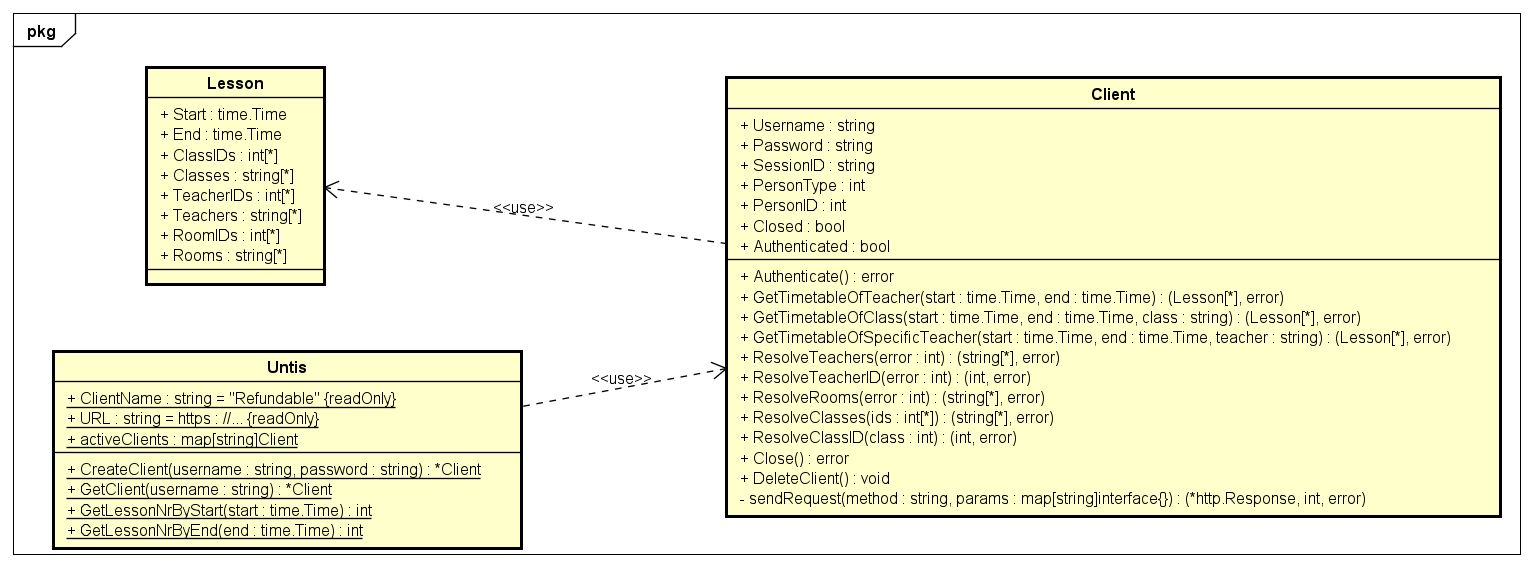
\includegraphics[width=\linewidth]{images/mbeier_konzept/Untis}
	\caption[\textit{Untis} \textit{API}-\textit{Client} \textit{UML}-Klassendiagramm]{\textit{UML}-Klassendiagramm des \textit{Untis} \textit{API}-\textit{Client} für das Abfragen von Stundenplaninformationen.}
	\label{fig:untis}
\end{figure}

\newpage

\subsubsection{LDAP}

\textit{LDAP} ist ein Zugriffsprotokoll um auf ein \textit{Active Directory} zugreifen zu können. In diesem wird im \textit{TGM} weitere Informationen zu den Lehrkräften und Schülern gespeichert. Um diese Daten einsehen zu können, muss man sich bei diesem Dienst anmelden, was mit den jeweils eigenen \textit{TGM}-\textit{Account} Zugangsdaten möglich ist. Dadurch ist die Anmeldung mit den \textit{TGM}-Nutzerdaten zu realisieren. Des Weiteren ist die Abfrage weiterer benötigter Daten hierdurch möglich. Der Ablauf einer solchen Interaktion über \textit{LDAP} wird in folgendem Flussdiagramm veranschaulicht.

\begin{figure}[H]
	\centering
	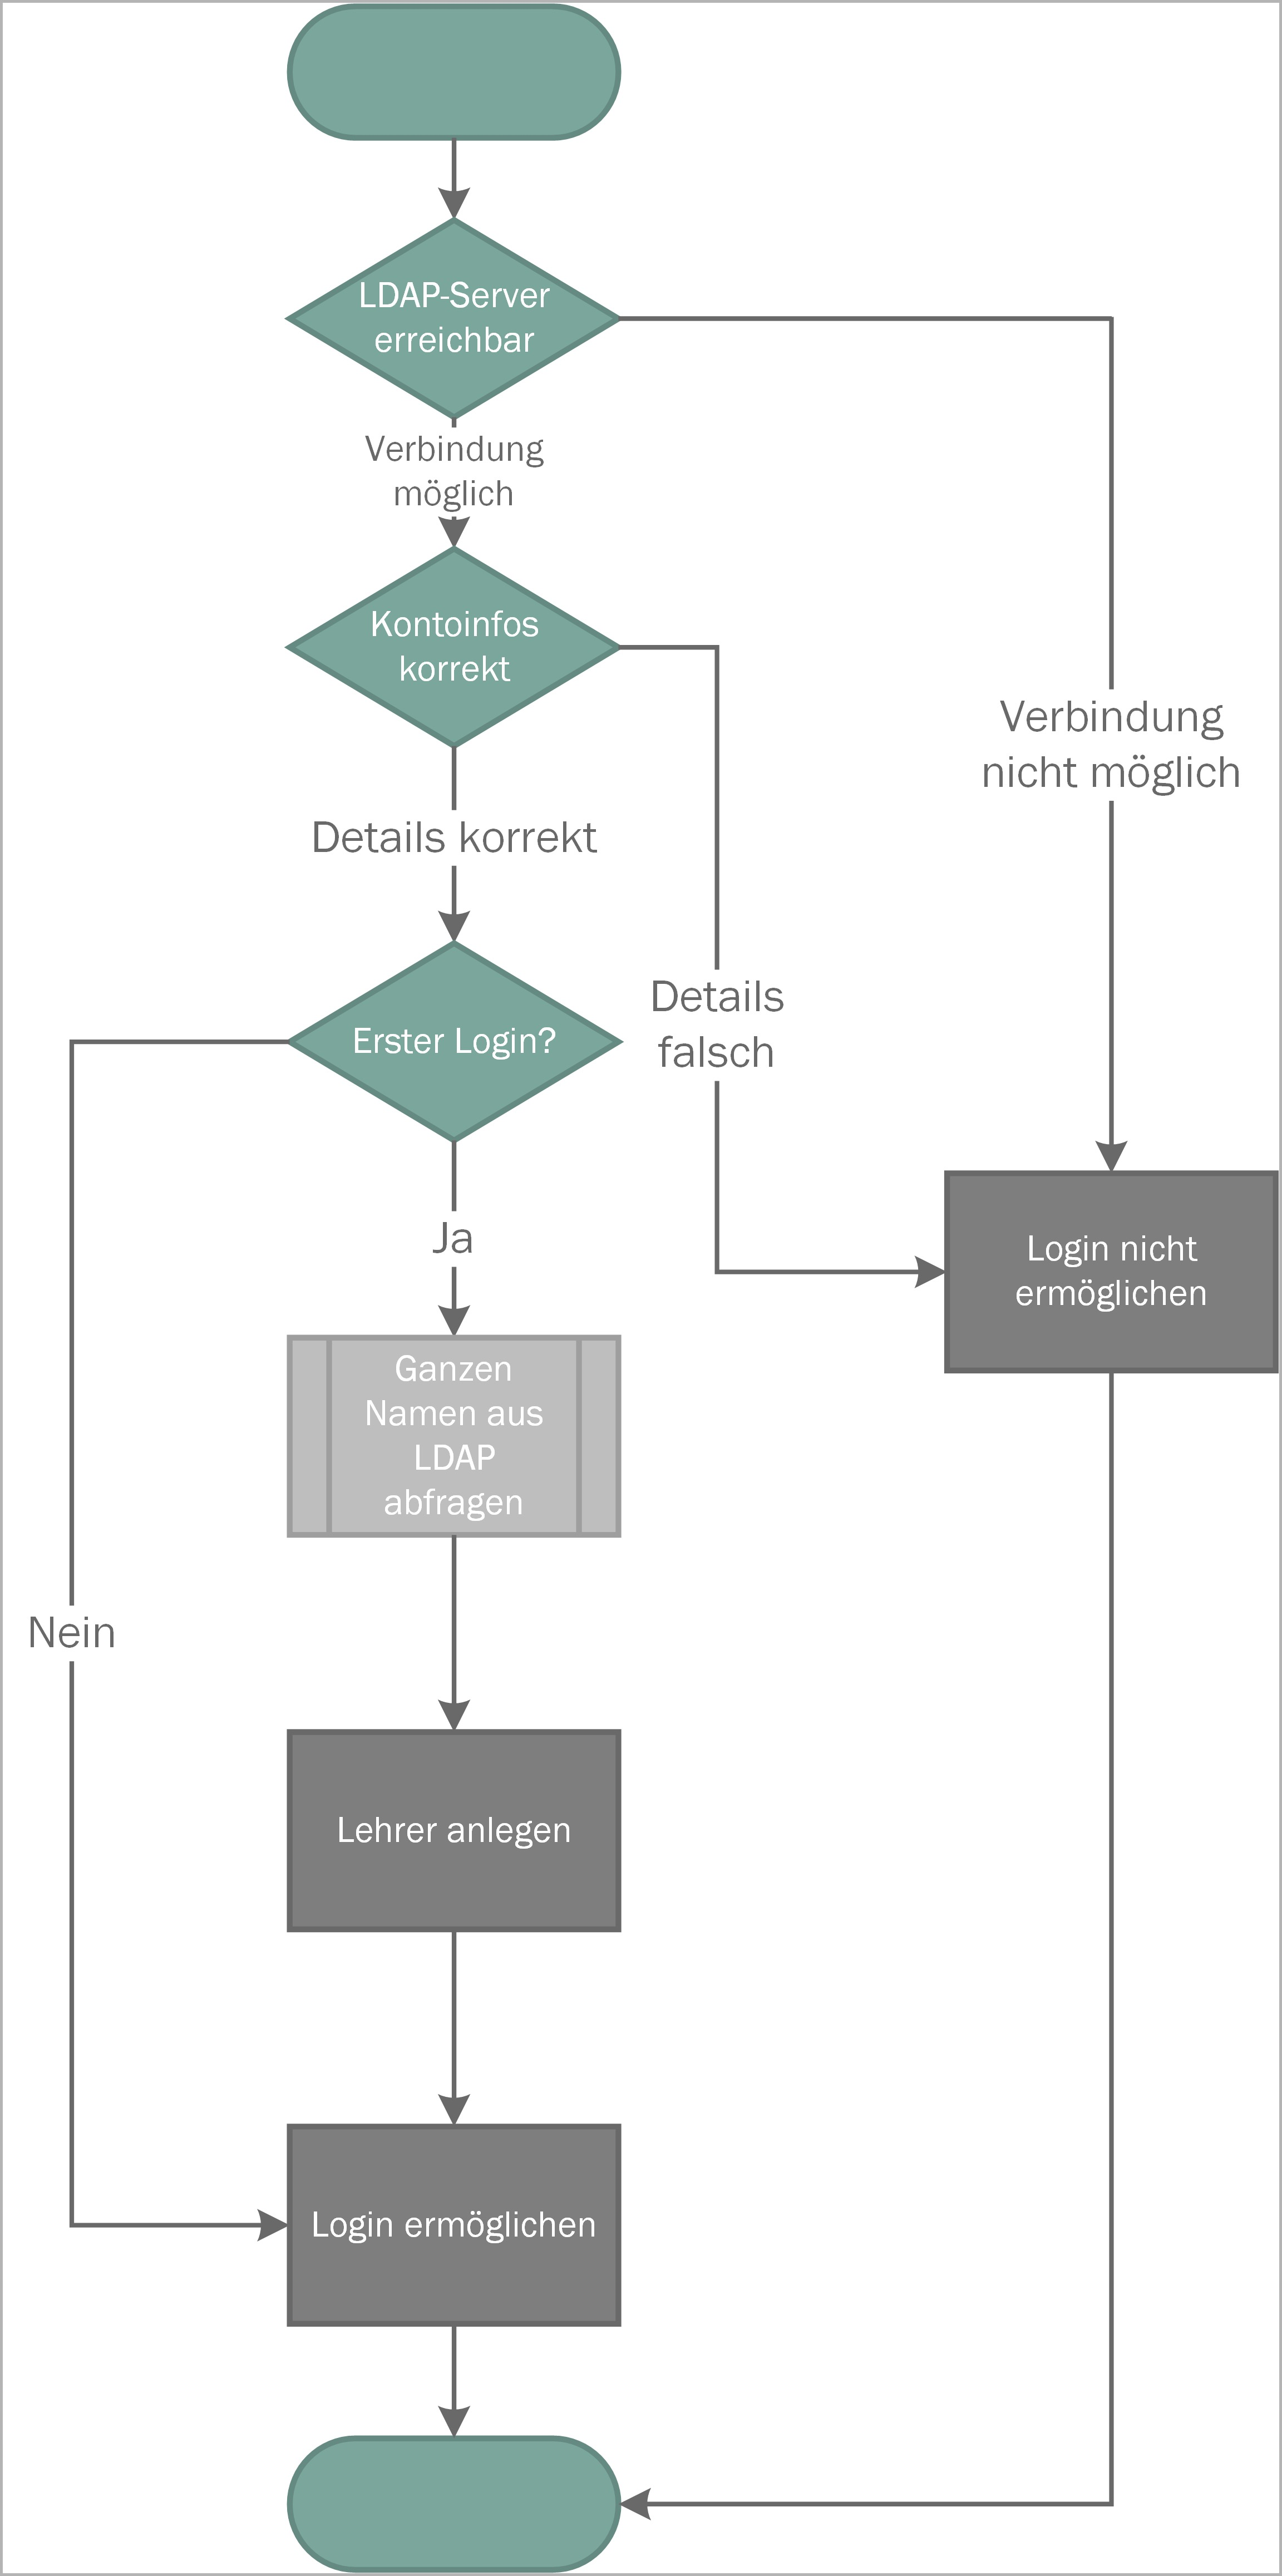
\includegraphics[width=0.5\linewidth]{images/mbeier_konzept/LDAP_border}
	\caption[Authentifizierung über \textit{LDAP}]{Authentifizierung über den \textit{TGM}-eigenen \textit{LDAP} \textit{Server}}
	\label{fig:ldapauthenticate}
\end{figure}

\newpage

Um jenen in \autoref{fig:ldapauthenticate} abgebildeten Ablauf einfach implementieren zu können, bietet sich folgender Aufbau eines \textit{LDAP}-\textit{Clients} an. Dieser kann hierbei die Zugangsdaten durch eine einfache Anmeldung beim Dienst verifizieren und auch die benötigten Daten, wie den kompletten Namen der Lehrkraft, beim Dienst abfragen.

\begin{figure}[H]
	\centering
	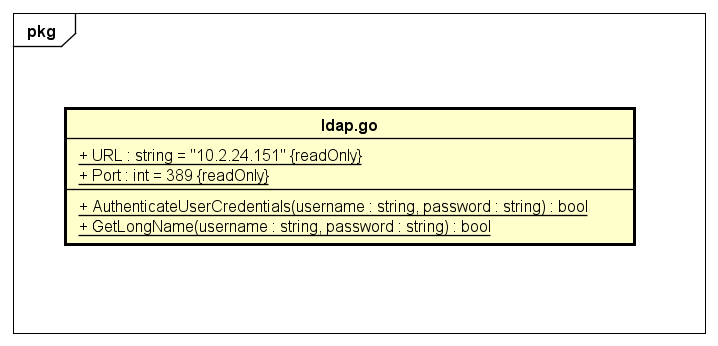
\includegraphics[width=\linewidth]{images/mbeier_konzept/LDAP}
	\caption[\textit{lLDAP} \textit{UML}-Klassendiagramm]{\textit{UML}-Klassendiagramm des \textit{LDAP} \textit{Packages} für die Authentifizierung von Lehrkräften}
	\label{fig:ldap}
\end{figure}

\newpage

\subsubsection{Dateierstellung}

Die Datei- und Formularerstellung ist die Hauptfunktion der Software. Das Generieren folgender Formulare wird unterstützt. Bei \enquote{Reiserechnung} und \enquote{Dienstreiseantrag} werden auf Grund des festgelegten \textit{Designs} auch eine \textit{Excel} Variante angeboten, in der dieses umgesetzt ist. Das Format steht hierbei für Hoch- oder Querformat, wobei \textit{Portrait} das Hochformat und \textit{Landscape} das Querformat ist.

\captionof{table}[Dateierstellung - Dateien]{Übersicht über die verschiedenen Dateien, die durch das \textit{Backend} erstellt werden.}	
\label{tbl:files}
\begin{table}
	\centering
	\begin{tabular}{|l|l|l|}
		\hline
		\multicolumn{1}{|c|}{\textbf{Formular}} & \multicolumn{1}{c|}{\textbf{Dateityp}} & \multicolumn{1}{c|}{\textbf{Format}} \\ \hline
		Abwesenheitsmeldung eines Jahrganges & PDF & Portrait \\ \hline
		Abwesenheitsmeldung eines Lehrers & PDF & Portrait \\ \hline
		Abgeltung für pädagogische Betreuung & PDF & Portrait \\ \hline
		Reiserechnung & PDF & Landscape \\ \hline
		Dienstreiseantrag & PDF & Portrait \\ \hline
		Reiserechnung & Excel & Landscape \\ \hline
		Dienstreiseantrag & Excel & Portrait \\ \hline
	\end{tabular}
\end{table}

~\\
Alle eigens generierten \textit{PDFs} sind jedenfalls mit einer Kopfzeile ausgestattet. In dieser ist in der linken Ecke das \textit{TGM}-Logo zu sehen, in der Mitte steht der Name des Formulars (siehe \autoref{tbl:files}) und rechts ein \textit{QR-Code}, welcher eine \textit{URL} beinhaltet, die den zugehörigen Antrag direkt im \textit{Frontend} öffnet.

\begin{figure}[H]
	\centering
	
\includegraphics[width=\linewidth]{images/mbeier_konzept/Kopfleiste_PDF_border}
	\caption[Kopfleiste \textit{PDF}-Datei]{Beispiel einer Kopfleiste in den vom \textit{Backend} generierten \textit{PDF}-Dateien}
	\label{fig:kopfleiste-pdf}
\end{figure}

